% Mini research note for simple profiles, stability, and transferability.
\documentclass[11pt]{article}
% Shared preamble for the research-note series.
% Create note-specific content in the per-note directory; keep common macros here.
\usepackage[margin=1in]{geometry}
\usepackage[T1]{fontenc}
\usepackage[utf8]{inputenc}
\usepackage{amsmath,amssymb}
\usepackage{booktabs,longtable,array}
\usepackage{graphicx}
\usepackage{float}
\usepackage{enumitem}
\usepackage{xcolor}
\usepackage{hyperref}
\usepackage{caption}
\usepackage{titlesec}
\hypersetup{colorlinks=true, linkcolor=blue!60!black, urlcolor=blue!60!black, citecolor=blue!60!black}
\setlist[itemize]{leftmargin=1.25em, itemsep=0.2em, topsep=0.3em}
\setlist[enumerate]{leftmargin=1.4em, itemsep=0.2em, topsep=0.3em}
\setlength{\parindent}{0pt}
\setlength{\parskip}{0.6em}
\newcommand{\statusbox}[2]{%
  \noindent\fcolorbox{black}{gray!10}{%
    \parbox{\dimexpr\linewidth-2\fboxsep-2\fboxrule\relax}{%
      \textbf{Status:} #1\\#2
    }%
  }
}

% Shared notation helpers for the research-note series.
\newcommand{\Jlin}{J}
\newcommand{\Jphys}{J_{\mathrm{phys}}}
\newcommand{\Jsurf}{J_{\mathrm{surf}}}
\newcommand{\JdB}{J_{\mathrm{dB}}}
\newcommand{\phiopt}{\phi_{\mathrm{opt}}}
\newcommand{\sigmathreedb}{\sigma_{3\mathrm{dB}}}
\newcommand{\Nt}{N_t}
\newcommand{\Nphi}{N_{\phi}}
\newcommand{\Lfiber}{L}
\newcommand{\Pcont}{P}
\newcommand{\band}{\mathcal{B}_{\mathrm{Raman}}}
\newcommand{\todoitem}[1]{\textcolor{red!70!black}{\textbf{TODO:} #1}}


\title{Simple Profiles, Universality, and Transferability}
\author{Fiber Raman Suppression Project}
\date{Evidence snapshot: 2026-04-26}

\begin{document}
\maketitle

\begin{abstract}
This note asks whether the project has found a simple, transferable
Raman-suppression phase mask, or whether the deepest masks are mostly local
optimizer artifacts. The answer is mixed and important. A very low-order
polynomial phase is the best simple transferable baseline, but it is shallow.
The deepest masks suppress Raman far more strongly, but they are fragile under
noise, pixelation, smoothing, and fiber transfer. The practical conclusion is
that ``deep,'' ``simple,'' and ``universal'' are different claims and must be
reported separately.
\end{abstract}

\section*{Claim Status}
\statusbox{settled comparison frame; not one universal mask}{The available
evidence supports a stable organizing story: low-order chirp-like profiles are
interpretable and transferable but shallow, while deep structured profiles are
local and hardware-sensitive. This note deliberately avoids the separate
long-fiber and multimode lanes, which still need their own evidence reviews.}

\section{Question and Thesis}

The baseline optimization problem asks for the phase mask \(\phi(\omega)\)
that gives the lowest Raman-band output fraction. This note asks a more
publishable question:
\[
    \text{Which masks are simple enough to explain and stable enough to test?}
\]

The reason is that a simulated phase mask can look impressive for the wrong
reason. A mask that gives \(-70\,\mathrm{dB}\) suppression but collapses after
\(0.05\,\mathrm{rad}\) of phase noise is not the same kind of result as a mask
that gives \(-26\,\mathrm{dB}\) suppression and transfers almost unchanged to a
different fiber. The first is a deep local optimum. The second is closer to a
general physical mechanism.

The thesis of this note is:
\[
    \text{the project has useful profile classes, not one magic phase mask.}
\]
The simple polynomial profile is the best presentation-friendly mask.
The deep simple-looking and cubic-basis masks are valuable, but they should be
presented as local high-performance masks unless they pass more stability and
hardware tests.

\subsection*{Intuition Check}

Spectral phase controls when different colors arrive in time. A simple
quadratic or cubic phase mostly stretches and delays parts of the pulse. That
can lower peak intensity and weaken Raman transfer. A highly detailed phase
can do much more, but it may also be tuned to one exact simulation grid,
fiber, and power. The scientific question is not just ``how low did \(J\)
go?'' It is also ``would this still work if I actually tried to use it?''

\section{Common Setup}

The controlled input is still
\[
    u_\omega(0;\phi)=u_{\omega,0}\exp(i\phi(\omega)),
\]
and the physical objective is the Raman-band energy fraction
\[
    \Jphys(\phi)
    =
    \frac{
    \sum_{\omega_k\in\band}|u_{\omega_k}(L;\phi)|^2\,\Delta\omega
    }{
    \sum_k |u_{\omega_k}(L;\phi)|^2\,\Delta\omega
    }.
\]
Lower values, reported as \(10\log_{10}\Jphys\), mean deeper suppression. The
forward model follows the standard nonlinear fiber propagation literature
\cite{agrawal2019,dudley2006,hult2007}. The physical motivation for simple
chirped phases is also consistent with pulse-stretching and chirped-pulse
ideas in ultrafast optics \cite{strickland1985,weiner2000}, and with Raman
red-shift physics in soliton propagation \cite{gordon1986,mitschke1986}.

\begin{figure}[H]
\centering
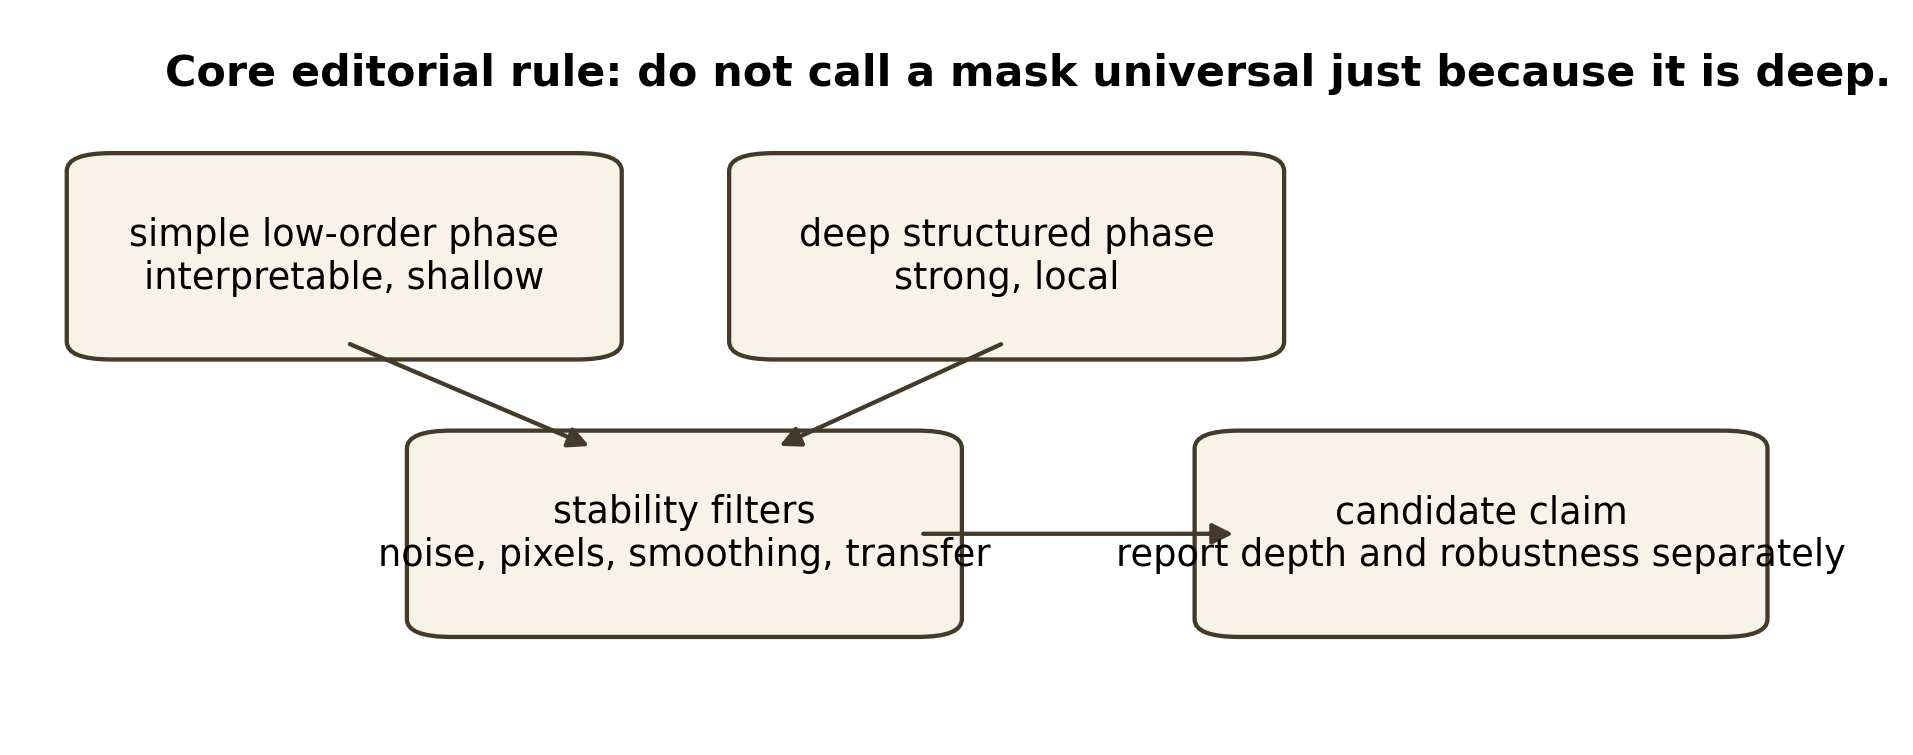
\includegraphics[width=0.92\linewidth]{figures/simple_transferability_workflow.png}
\caption{Workflow for judging simple and transferable masks. The note treats
depth, interpretability, robustness, and transfer as separate axes rather than
collapsing everything into one ``best'' number.}
\end{figure}

\section{Math Delta: What Counts as Simple?}

A phase mask is not automatically simple just because it looks smooth. First,
we remove the two gauge-like pieces that do not represent meaningful pulse
shaping for this objective:
\[
    \phi_{\perp}
    =
    (I-P_{\mathcal{G}})\phi,
    \qquad
    \mathcal{G}=\operatorname{span}\{1,\omega-\bar{\omega}\}.
\]
The constant term is global phase. The linear-in-frequency term is mainly a
time shift. After removing these, we can ask whether the remaining shape is
well described by a low-order family.

The simplest tested family is a polynomial expansion on the active spectral
band:
\[
    \phi_{\perp}(\Omega)
    \approx
    a_2\Omega^2+a_3\Omega^3+\cdots+a_p\Omega^p,
    \qquad
    \Omega=\frac{\omega-\omega_0}{\Delta\omega_{\mathrm{band}}}.
\]
The quadratic term is group-delay dispersion-like chirp. The cubic term adds
third-order timing asymmetry. Higher terms can fit more structure, but they
become harder to interpret and usually less transferable.

The project also uses rough complexity checks:
\[
    \mathrm{TV}(\phi)=\sum_i|\phi_{i+1}-\phi_i|,
    \qquad
    \mathrm{curvature}(\phi)=\sum_i|\phi_{i+1}-2\phi_i+\phi_{i-1}|.
\]
These are not physics laws. They are audits that help separate compact masks
from fine-scale masks.

\subsection*{Intuition Check}

Linear algebraically, this is projection plus fitting. First project away the
boring directions: constant phase and timing shift. Then ask, ``can the part
that remains be described with a few basis vectors?'' If yes, the mask is
compact enough to explain cleanly. If no, it may still be real, but it needs stronger
stability evidence.

\section{Transfer and Robustness Metrics}

The native objective is only one metric. A profile is also tested by how it
survives changes:
\[
    \Delta_{\mathrm{transfer}}
    =
    J_{\mathrm{new\ setup}}(\phi_{\mathrm{fixed}})
    -
    J_{\mathrm{native}}(\phi_{\mathrm{fixed}}).
\]
A small transfer gap means the same fixed mask still helps in the new setup.
For phase noise, the profile is perturbed as
\[
    \phi_{\sigma}=\phi+\epsilon,
    \qquad
    \epsilon_i\sim\mathcal{N}(0,\sigma^2),
\]
and the loss is measured relative to the unperturbed mask. The
\(3\,\mathrm{dB}\) noise width, \(\sigma_{3\mathrm{dB}}\), is the approximate
noise level where the mask loses \(3\,\mathrm{dB}\) of suppression.

Hardware-like probes include active-band pixel resampling, smoothing, and
wrapped finite-bit phase masks. These are not perfect lab models, but they are
good filters: a candidate that fails badly under these probes is not ready to
be called universal.

\subsection*{Intuition Check}

If the mask only works when every pixel is exactly right, it is probably a
simulation-specific key, not a general lockpick. Transfer and robustness tests
ask whether the same idea still works after small real-world changes.

\section{Implementation Surface}

\begin{center}
\small
\begin{tabular}{p{0.34\linewidth}p{0.56\linewidth}}
\toprule
\textbf{Component} & \textbf{Role} \\
\midrule
\texttt{simple\_profile\_driver.jl} & Generates the original simple-profile
baseline, perturbation, and transfer studies. \\
\texttt{simple\_profile\_metrics.jl} & Computes gauge-fixed simplicity metrics
such as stationary points, total variation, and curvature. \\
\texttt{sweep\_simple\_param.jl} & Scans low-resolution phase parameterizations
for simple non-dominated candidates. \\
Stability probe driver & Applies transfer, phase-noise, pixelation,
smoothing, and wrapped-mask probes to saved candidates. \\
Standard-image builder & Produces phase diagnostics and spectral-evolution
images for representative candidates. \\
\bottomrule
\end{tabular}
\end{center}

The human-facing figures in this note are copied or summarized from those
candidate-standard-image bundles and stability tables.

\section{Representative Candidate Classes}

\begin{figure}[H]
\centering
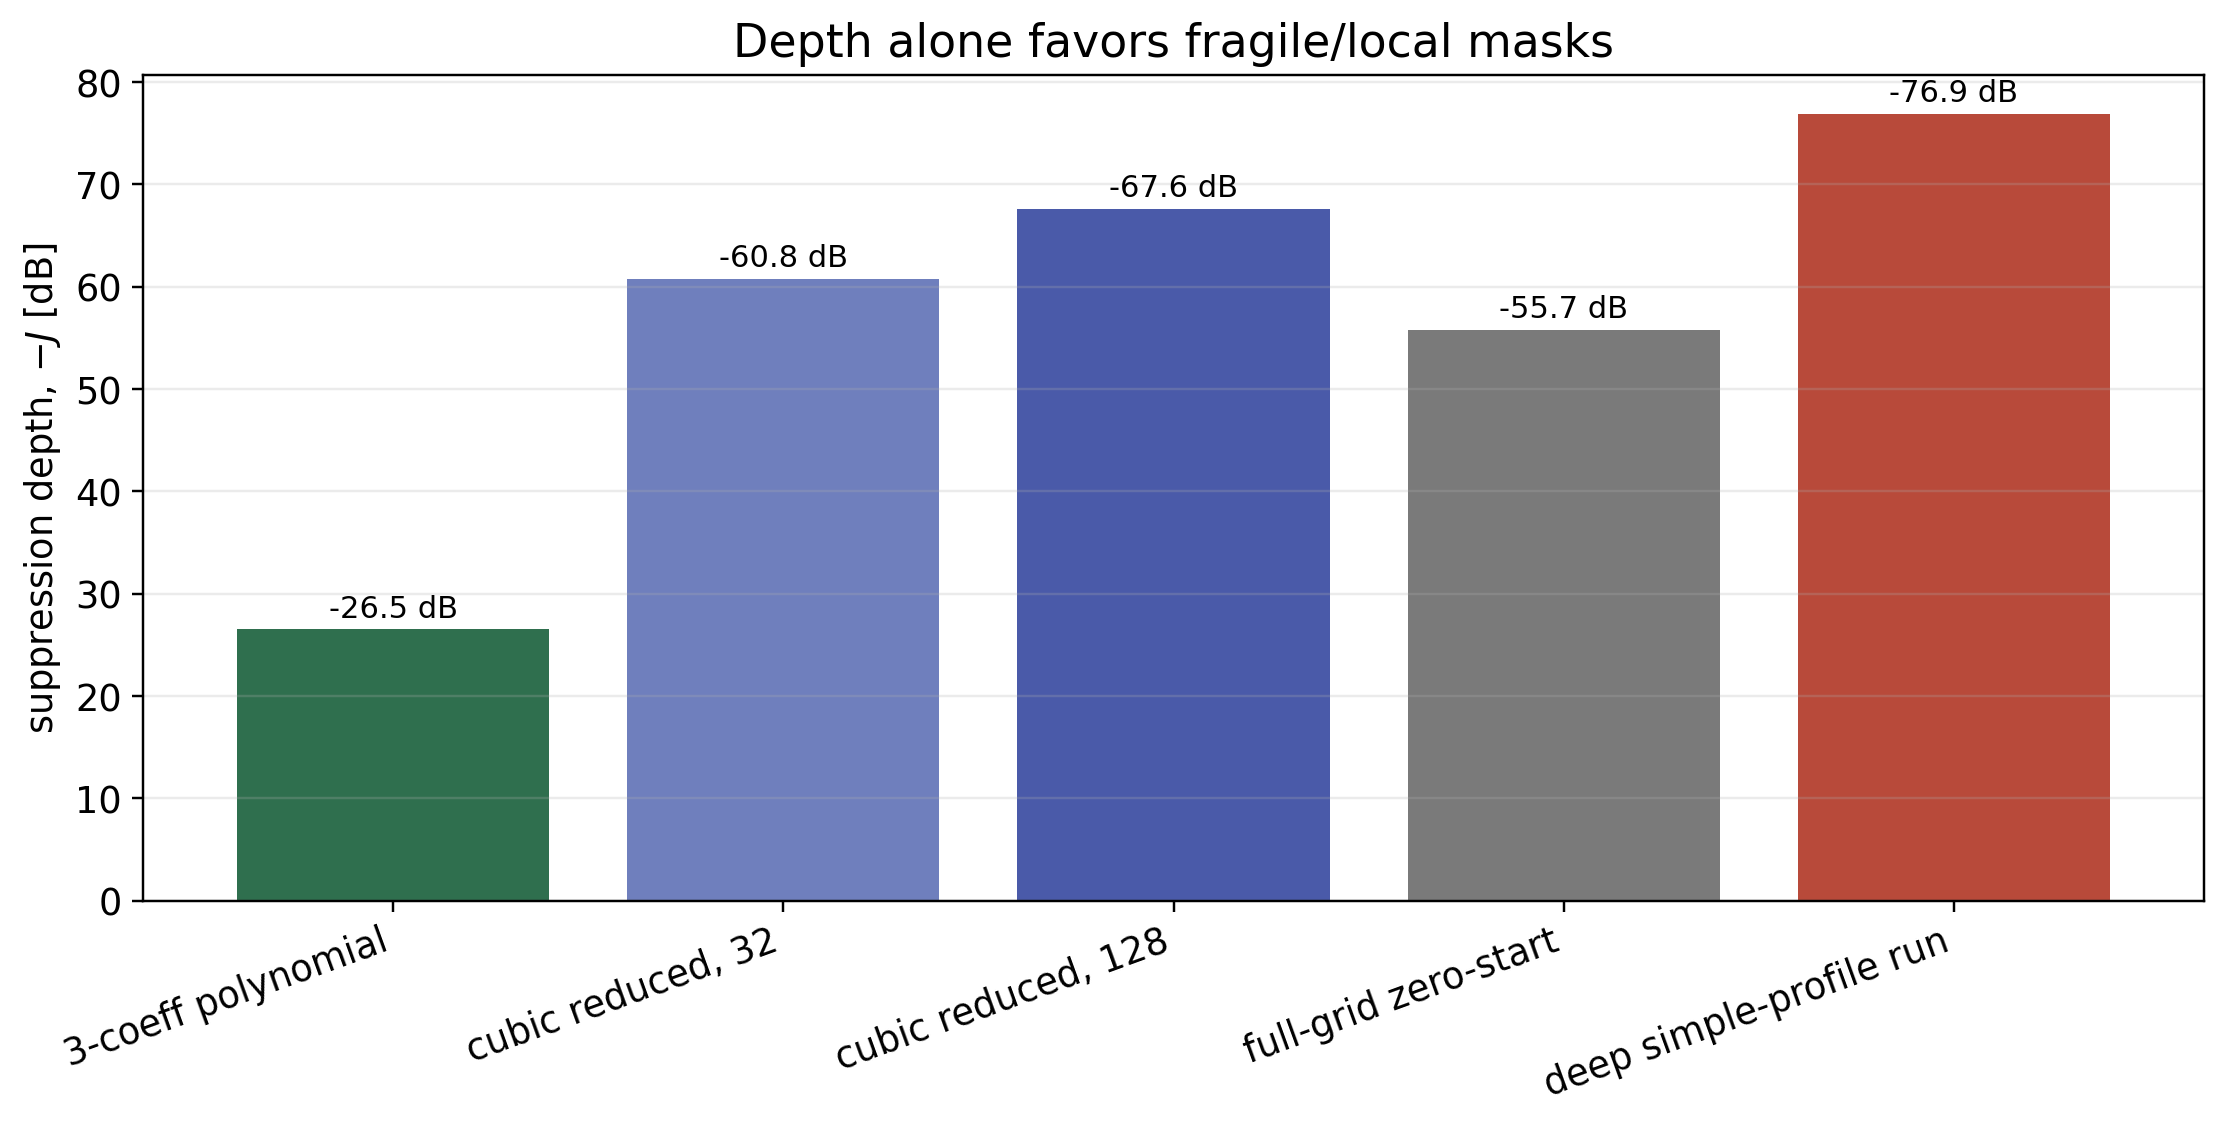
\includegraphics[width=0.90\linewidth]{figures/native_depth_comparison.png}
\caption{Native depth comparison. The deepest masks are not the same masks
that transfer or survive hardware-like perturbations best.}
\end{figure}

\begin{center}
\footnotesize
\begin{tabular}{>{\raggedright\arraybackslash}p{0.30\linewidth}
                >{\raggedright\arraybackslash}p{0.15\linewidth}
                >{\raggedright\arraybackslash}p{0.20\linewidth}
                >{\raggedright\arraybackslash}p{0.24\linewidth}}
\toprule
\textbf{Candidate class} & \textbf{native \(J\)} & \textbf{transfer gap} & \textbf{reading} \\
\midrule
3-coefficient polynomial & \(-26.50\,\mathrm{dB}\) & \(0.29\,\mathrm{dB}\) to HNLF & best simple-transfer baseline \\
cubic reduced, 32 coeff. & \(-60.77\,\mathrm{dB}\) & \(16.51\,\mathrm{dB}\) & deep local structured mask \\
cubic reduced, 128 coeff. & \(-67.60\,\mathrm{dB}\) & \(21.50\,\mathrm{dB}\) & deeper but more local \\
full-grid zero-start & \(-55.75\,\mathrm{dB}\) & \(11.47\,\mathrm{dB}\) & robustness reference; not simple \\
deep simple-looking run & \(-76.86\,\mathrm{dB}\) & not kept as fixed-transfer claim & deepest but fragile \\
\bottomrule
\end{tabular}
\end{center}

The table is the core story. The 3-coefficient polynomial is nowhere near the
deepest native result, but it transfers almost unchanged across a fiber change
in the available metrics. The deep candidates are much stronger at their home
setup, but their transfer gaps are large or unproven.

\subsection*{Intuition Check}

The polynomial mask is like a simple rule of thumb: not perfect, but easy to
explain and surprisingly portable. The deep masks are like specialized keys:
excellent in one lock, but not automatically useful in another.

\section{Depth Versus Transfer}

\begin{figure}[H]
\centering
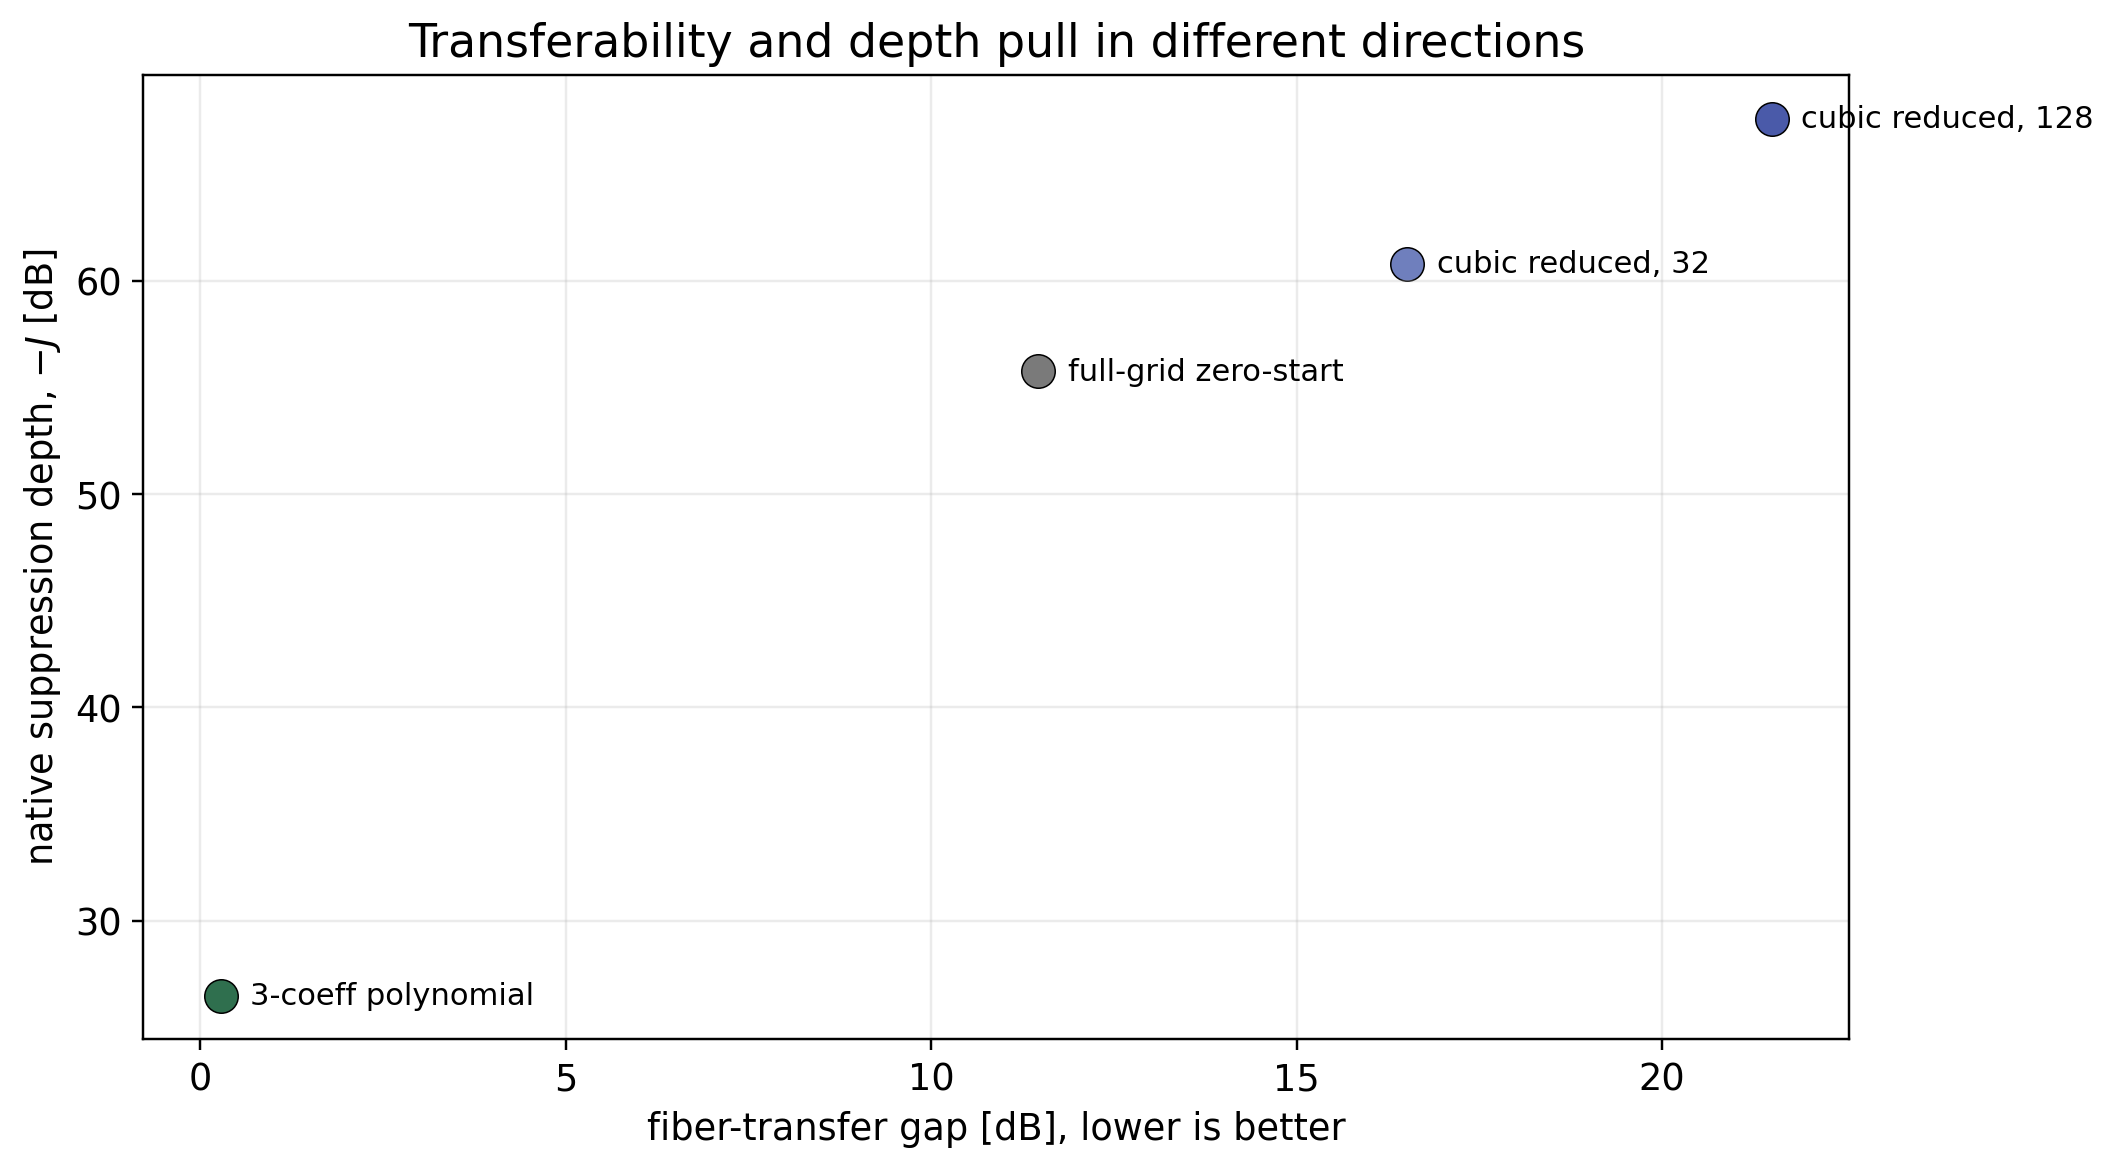
\includegraphics[width=0.86\linewidth]{figures/depth_transfer_tradeoff.png}
\caption{Depth-transfer tradeoff. The simple polynomial is shallow but
transfers well; deeper cubic and full-grid masks lose much more performance
when evaluated in a different fiber setting.}
\end{figure}

This figure is why the word ``universal'' has to be used carefully. A universal
mask would ideally sit in the upper-left: deep suppression and small transfer
gap. The available profiles do not yet give that ideal point. Instead, the
project has a shallow transferable mechanism and several deep local mechanisms.

\subsection*{Intuition Check}

If you had to explain one profile clearly to a new lab member, start with the
low-order polynomial. If you had to show the deepest simulation
result, use the deep profiles. Those are different presentation goals.

\section{Hardware and Stability Filters}

\begin{figure}[H]
\centering
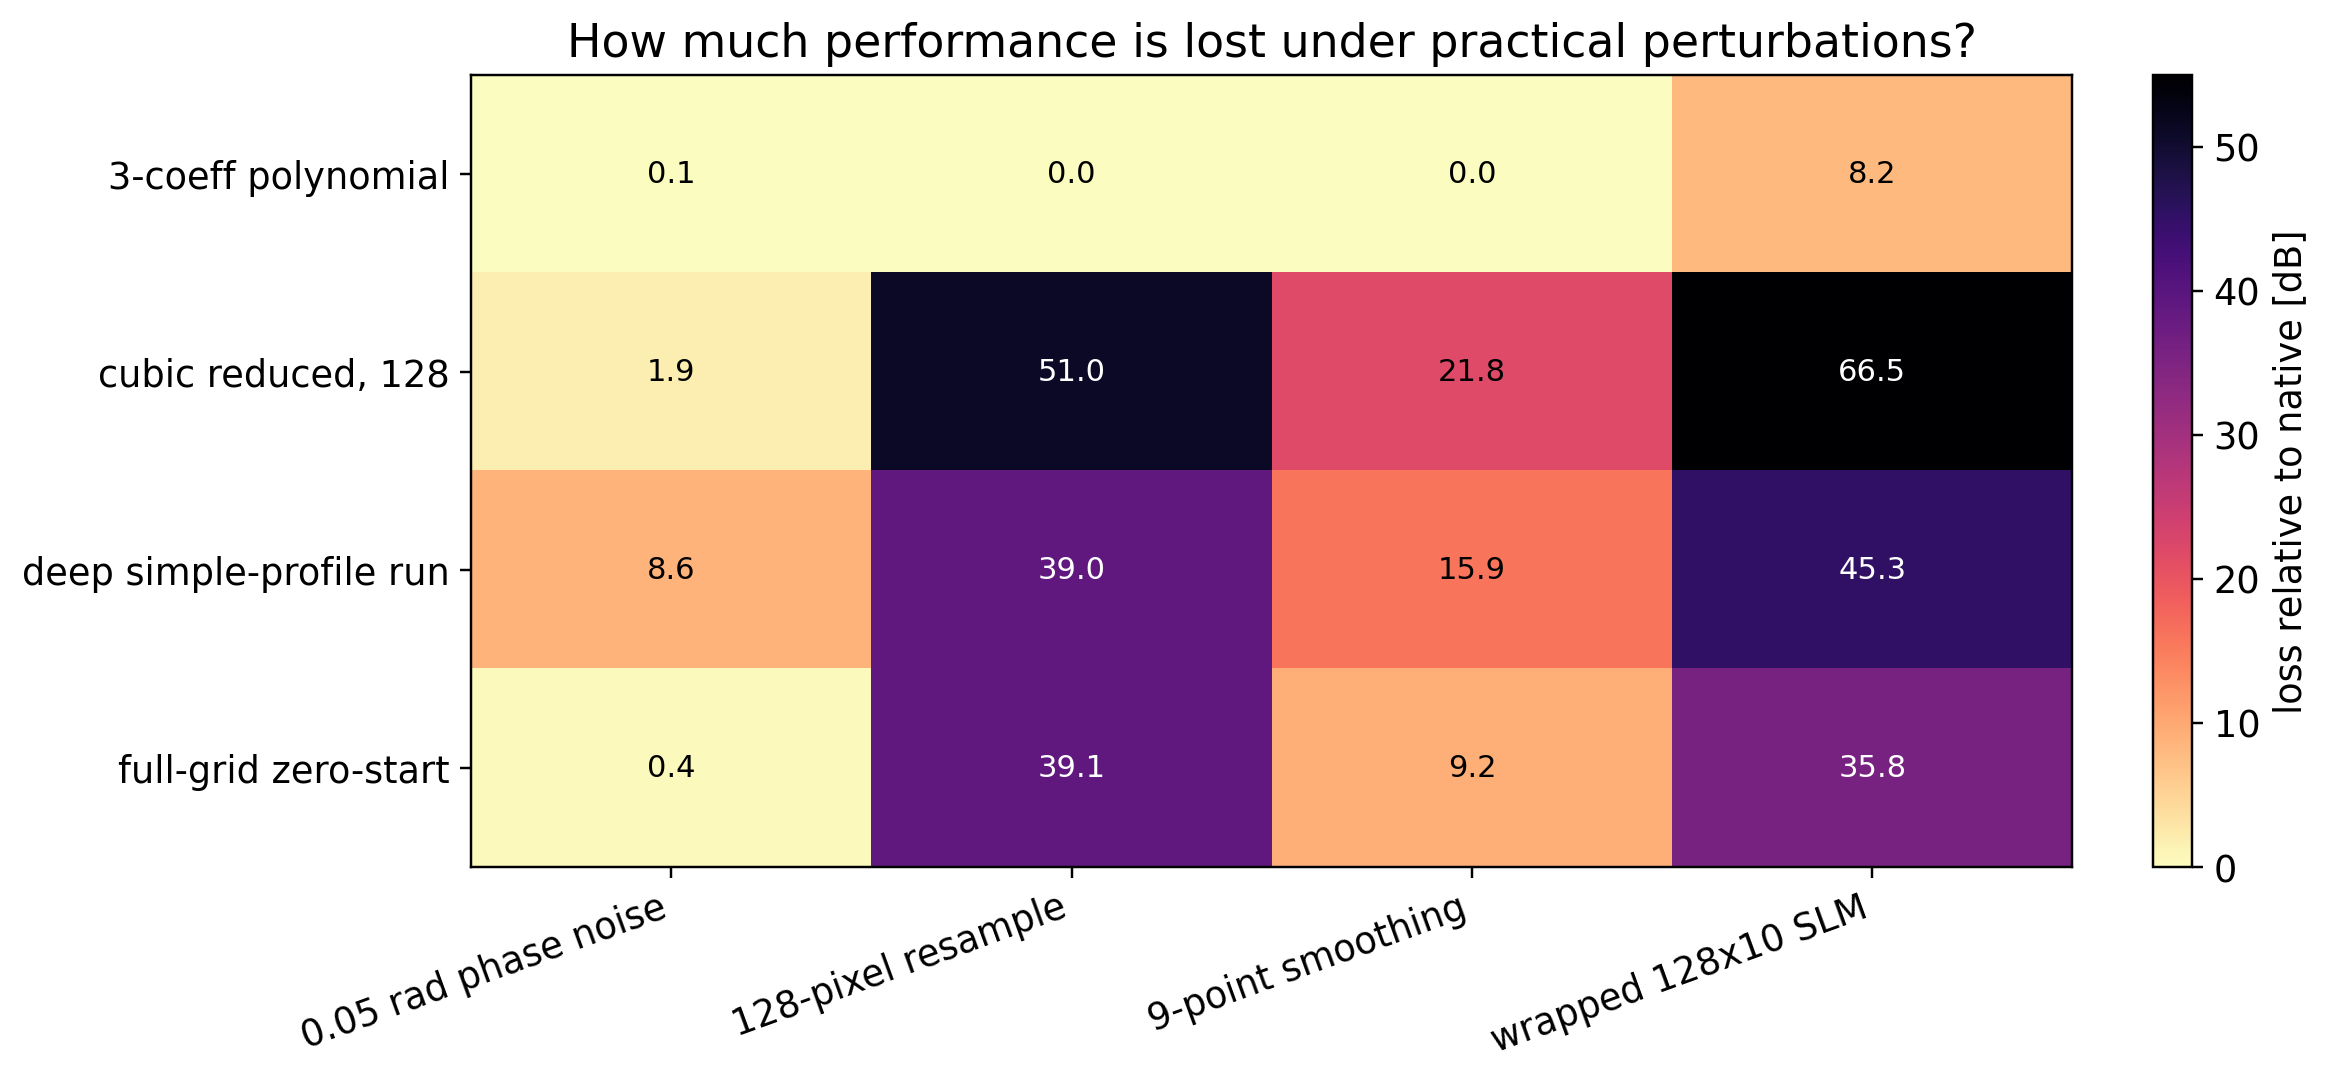
\includegraphics[width=0.92\linewidth]{figures/hardware_robustness_loss_matrix.png}
\caption{Loss under practical perturbations. Numbers are dB lost relative to
the native candidate. The simple polynomial survives noise, pixel resampling,
and smoothing well; the deep masks lose tens of dB under several hardware-like
filters.}
\end{figure}

The low-order polynomial loses almost nothing under \(0.05\,\mathrm{rad}\)
Gaussian phase noise, active-band pixel resampling, or active-band smoothing.
Its wrapped finite-bit mask loss is larger, but still far smaller than the
losses for the deep structured masks in the same probe. The deep
simple-looking run loses about \(8.6\,\mathrm{dB}\) under
\(0.05\,\mathrm{rad}\) noise and tens of dB under pixelation or wrapping.

This does not make the deep masks useless. It means they need either better
hardware-aware optimization or a different claim: ``deep simulated local
profile,'' not ``universal fixed mask.''

\subsection*{Intuition Check}

Robustness is the difference between a trick and a tool. A trick can work
beautifully once. A tool still works when the setup is slightly imperfect.

\clearpage
\section{Representative Result Pages}

The pages below pair each phase diagnostic with the corresponding heat map.
This makes the comparison visual: what the mask looks like, and how the
propagation changes.

\begin{figure}[p]
\centering

\includegraphics[height=0.47\textheight]{figures/no_optimization_phase_diagnostic.png}
\par\vspace{0.5em}
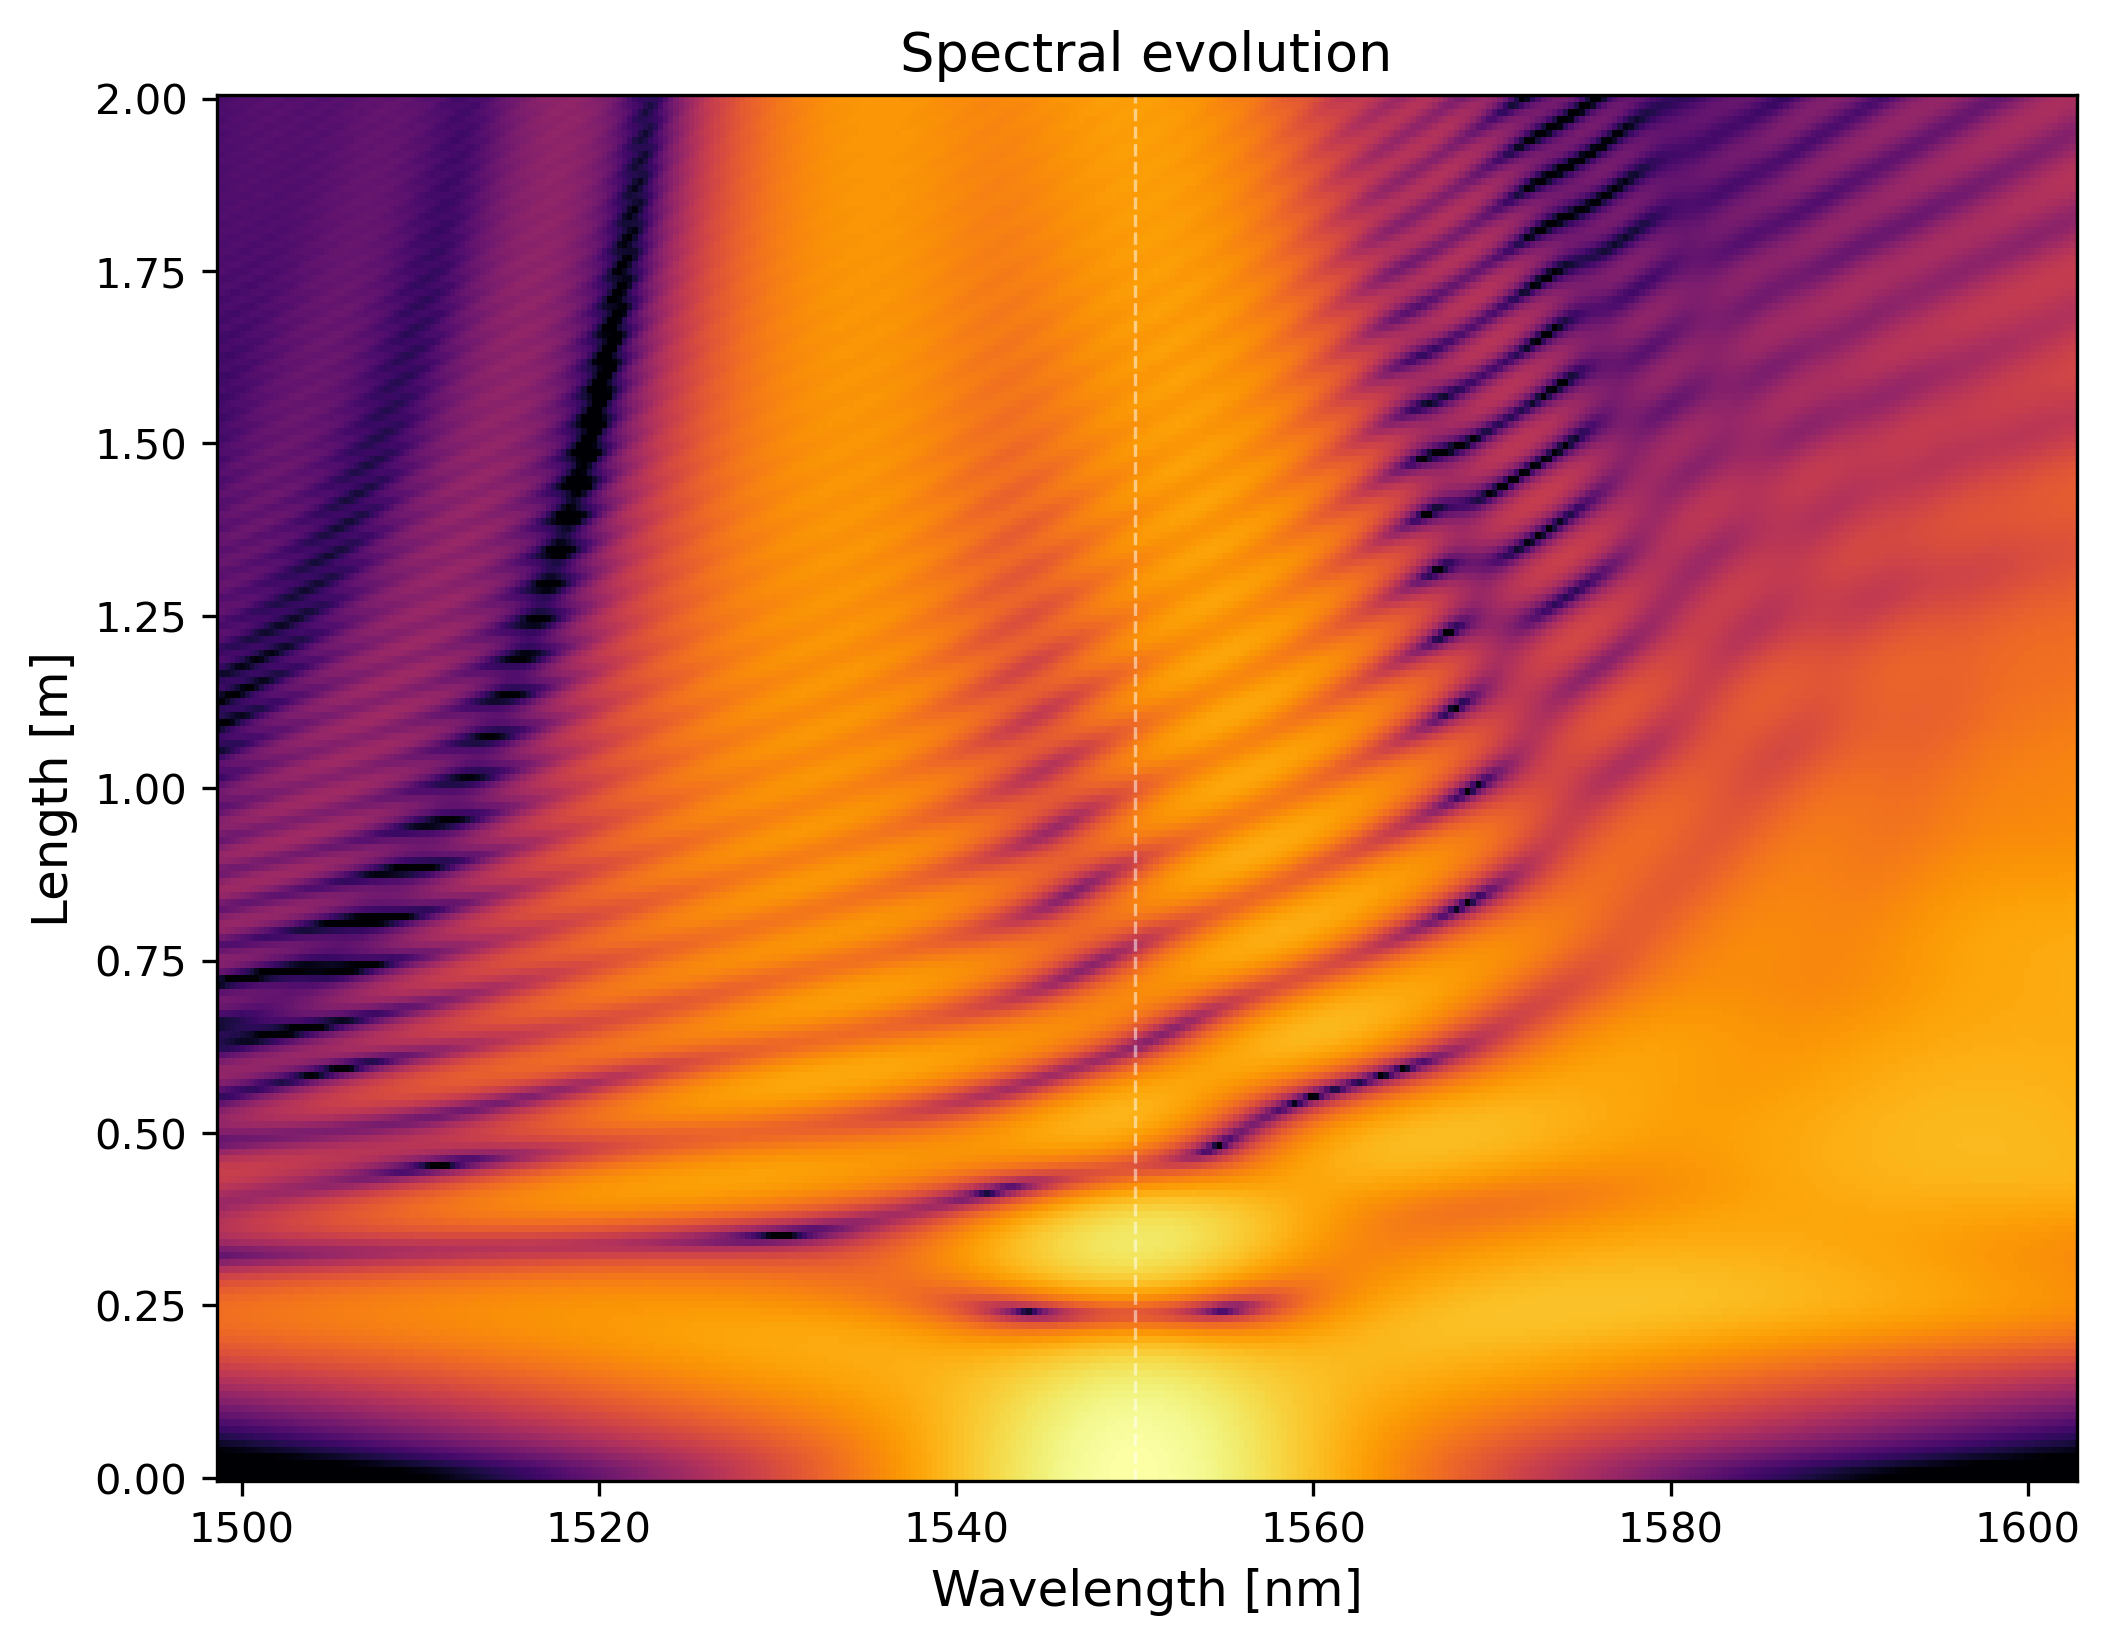
\includegraphics[height=0.31\textheight]{figures/no_optimization_evolution.png}
\caption{No-optimization control. The phase is flat, and the heat map shows
the unshaped propagation reference used to judge whether a shaped candidate is
actually changing Raman-band growth.}
\end{figure}

\begin{figure}[p]
\centering
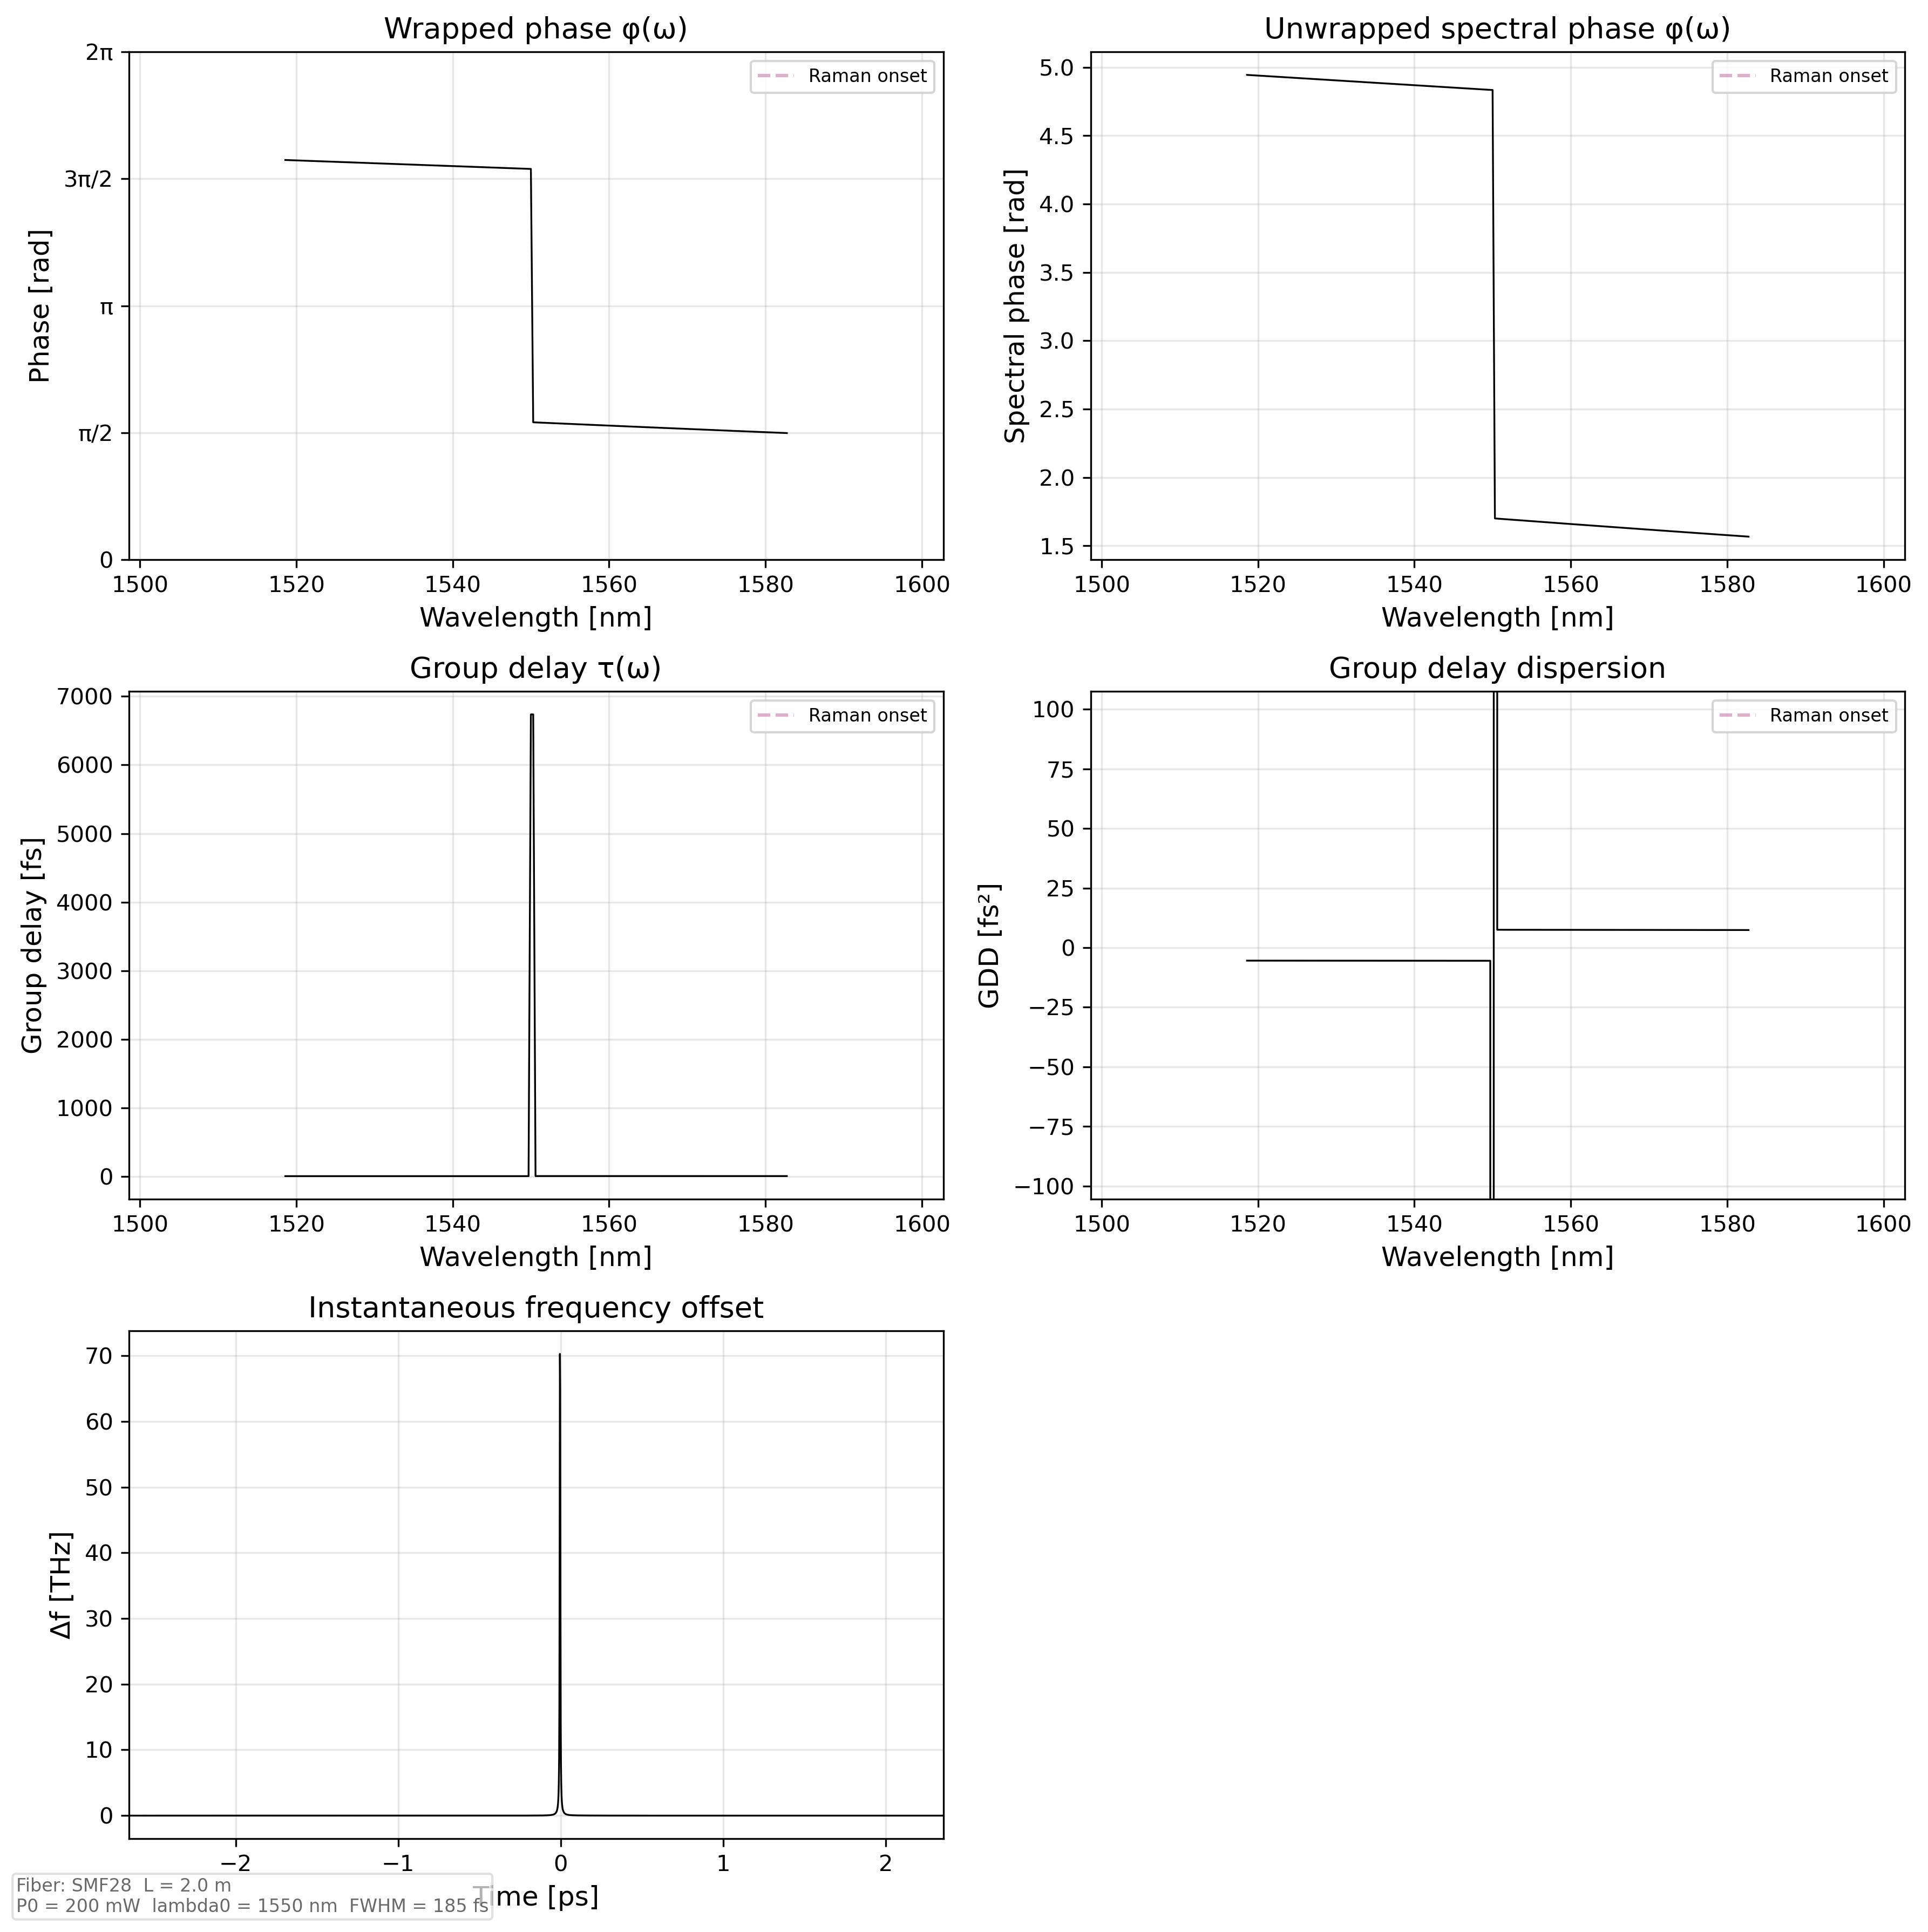
\includegraphics[height=0.47\textheight]{figures/transferable_polynomial_phase_diagnostic.png}
\par\vspace{0.5em}
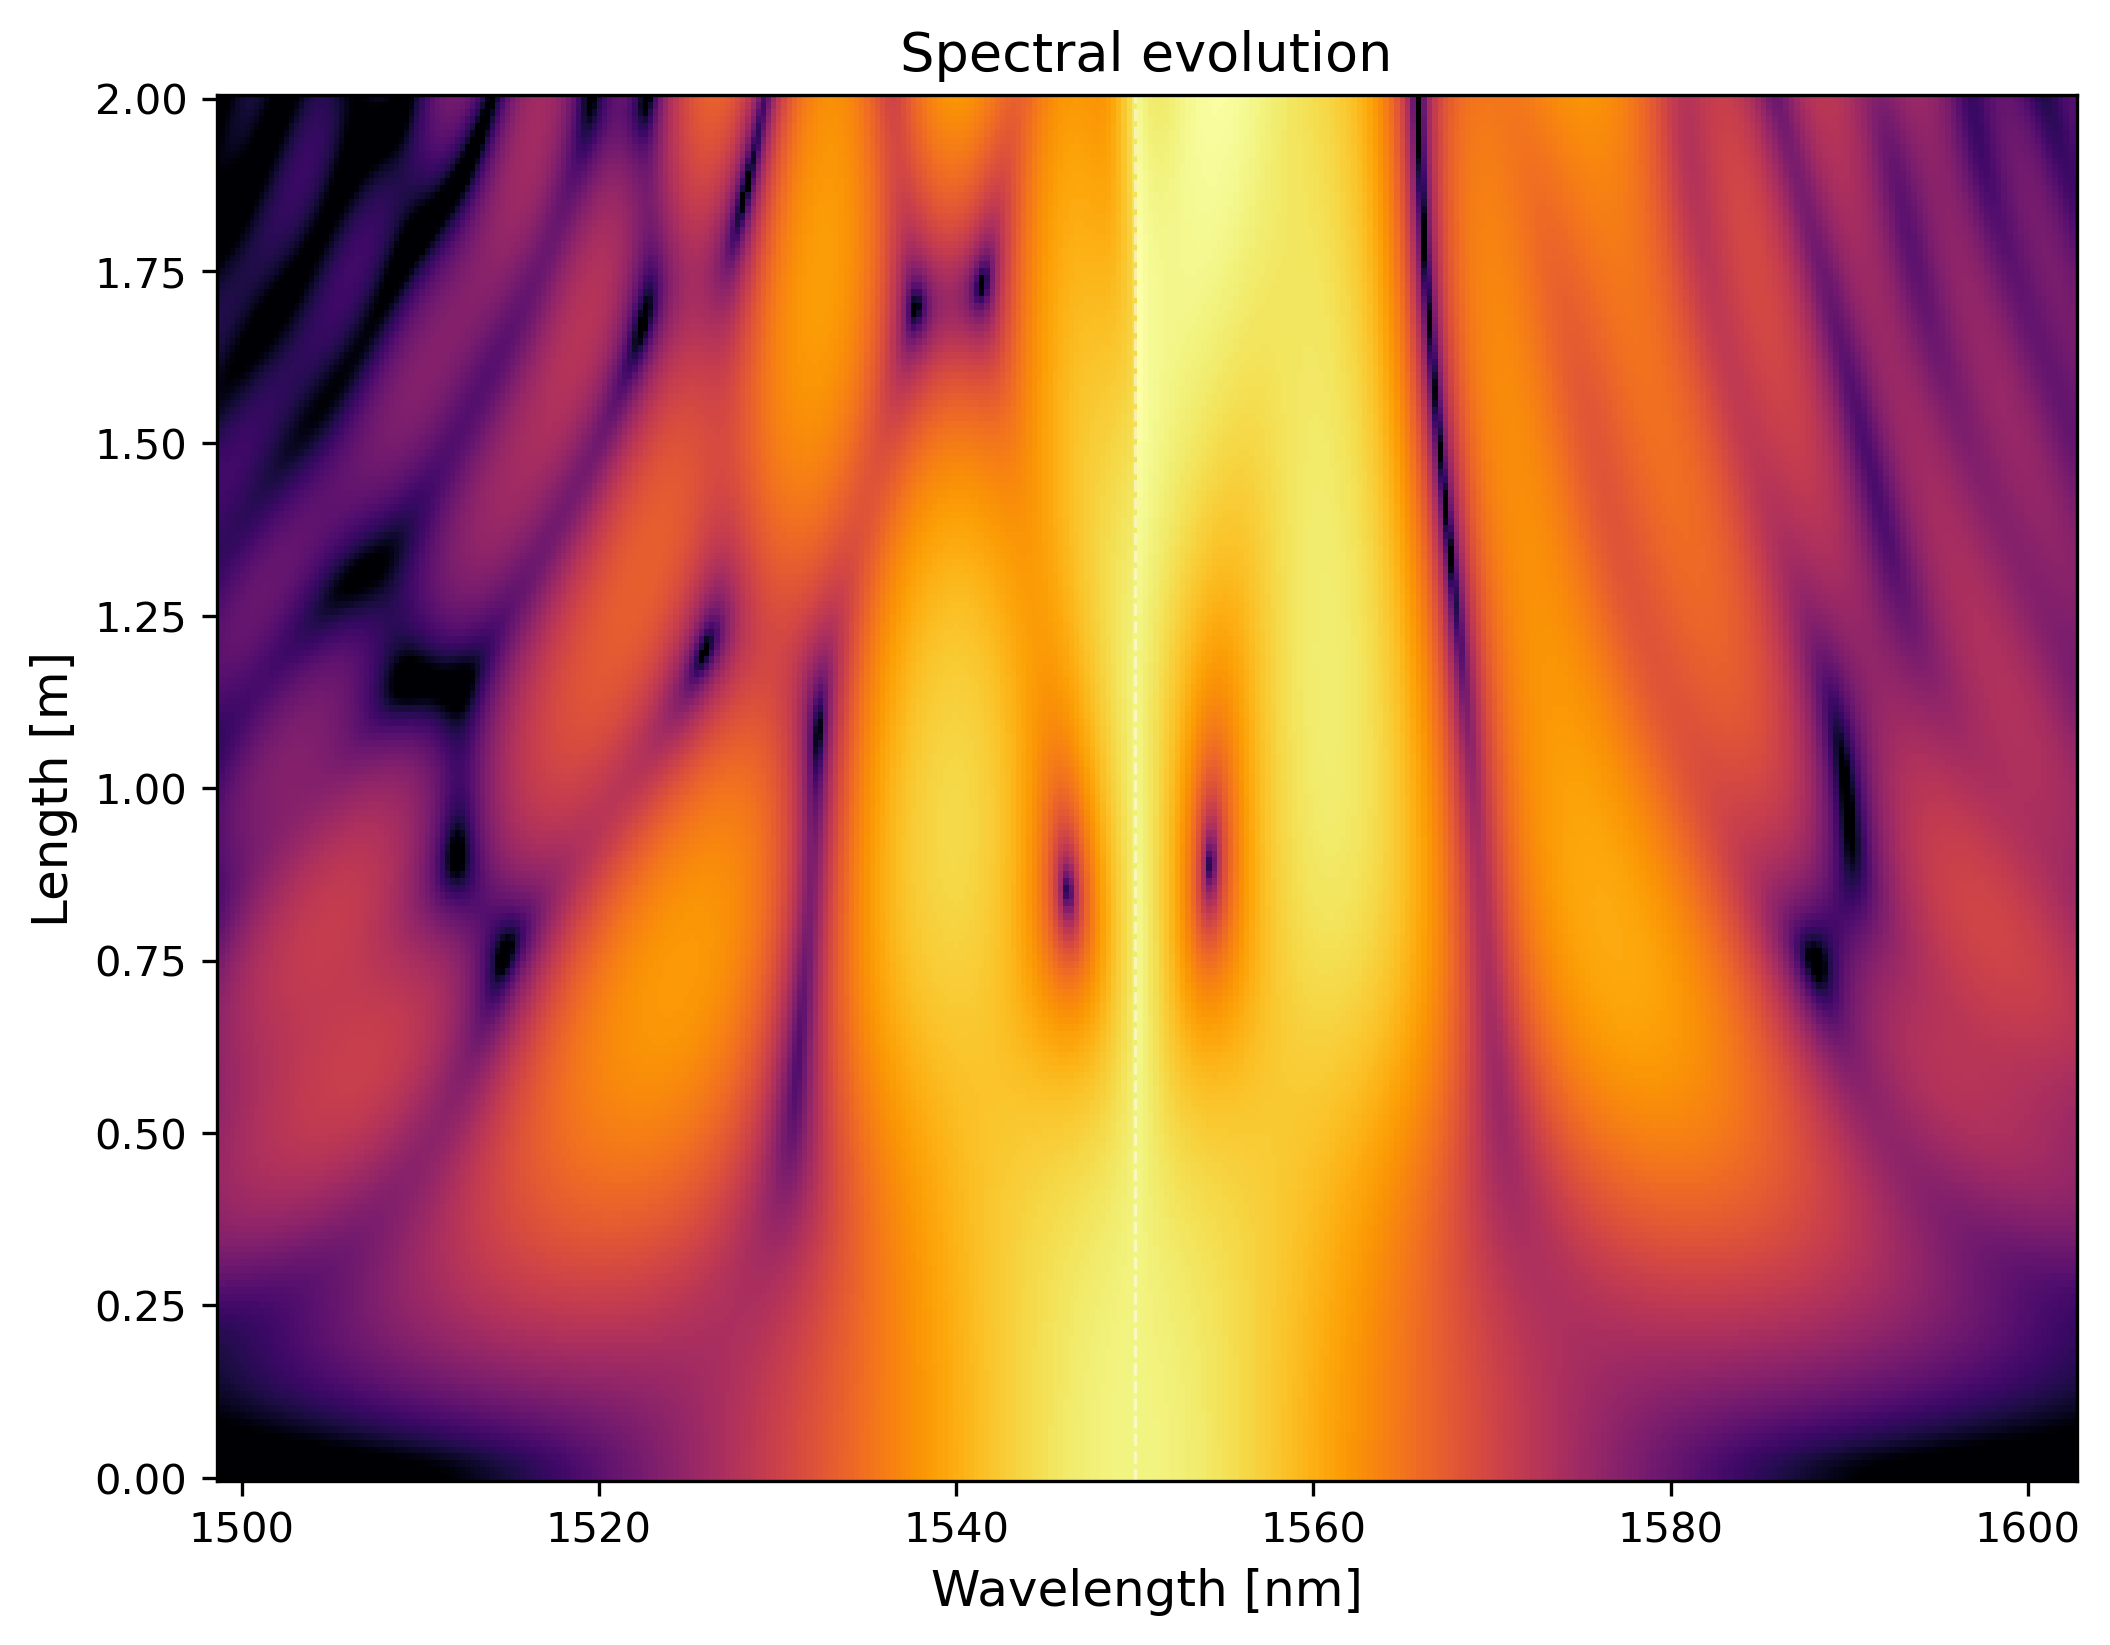
\includegraphics[height=0.31\textheight]{figures/transferable_polynomial_evolution.png}
\caption{Simple transferable polynomial mask. The suppression is shallower
than the deep masks, but the phase is compact and the available transfer
metrics are much stronger.}
\end{figure}

\begin{figure}[p]
\centering
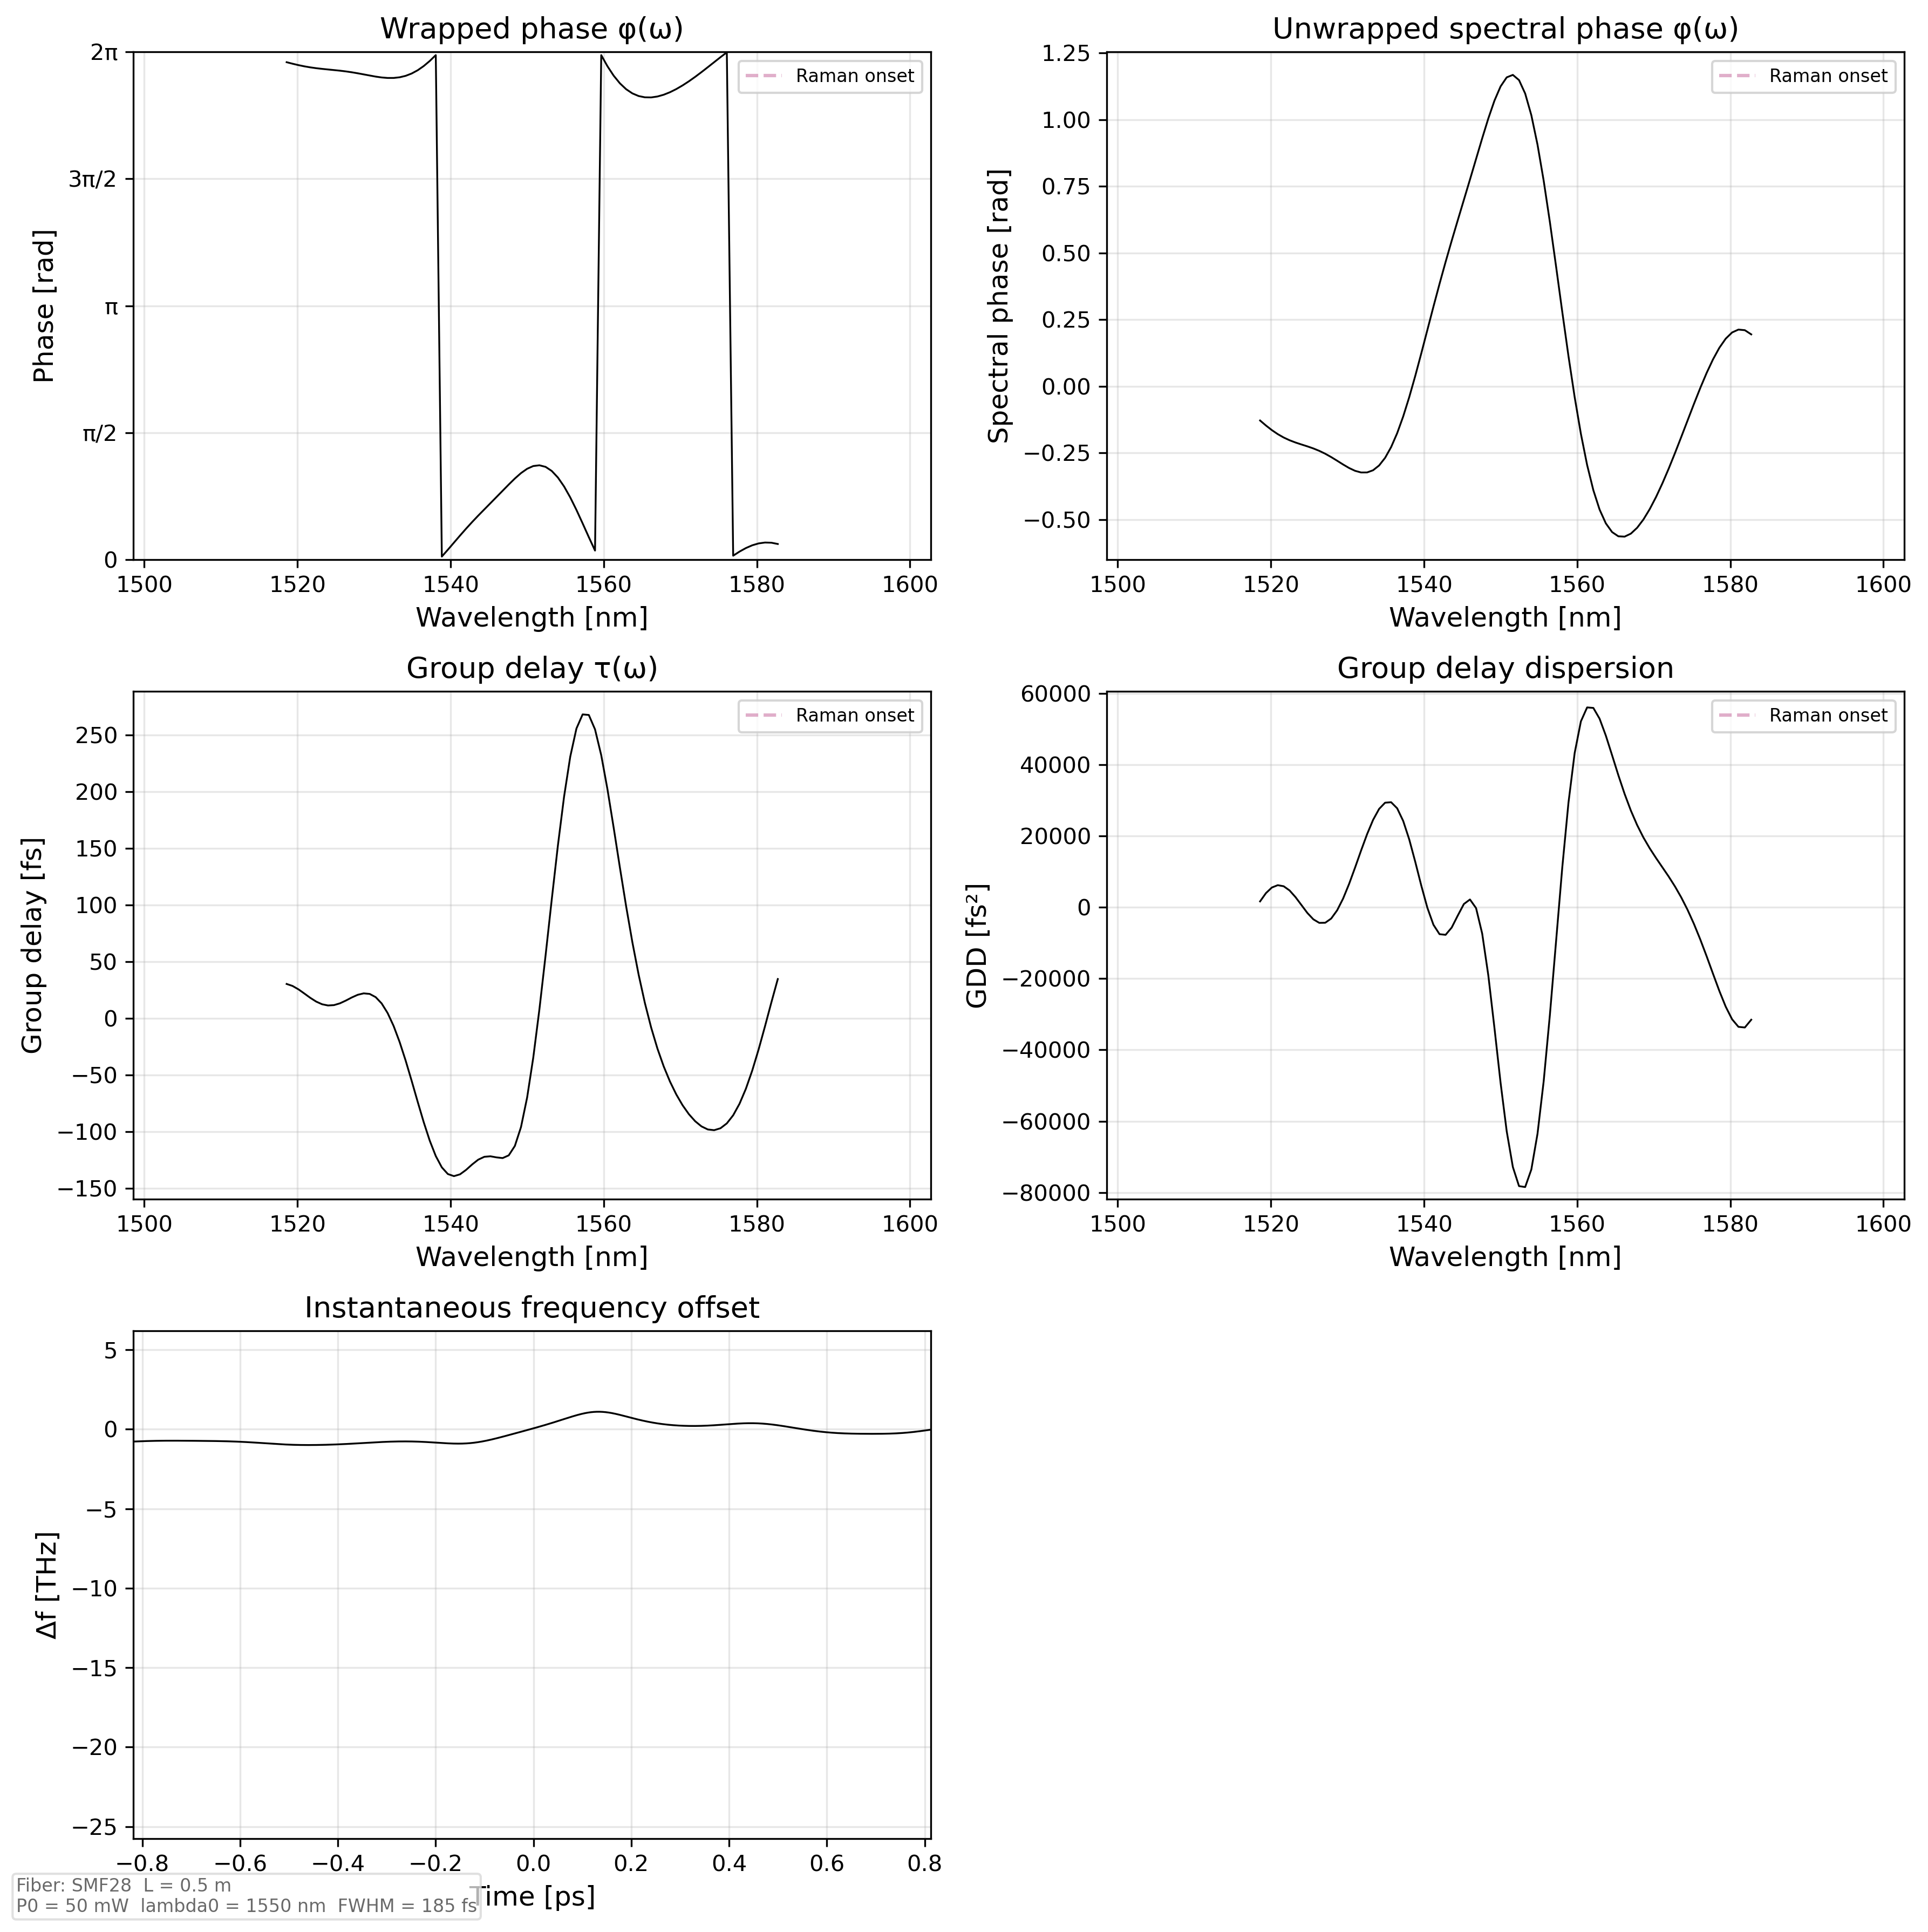
\includegraphics[height=0.47\textheight]{figures/deep_simple_profile_phase_diagnostic.png}
\par\vspace{0.5em}
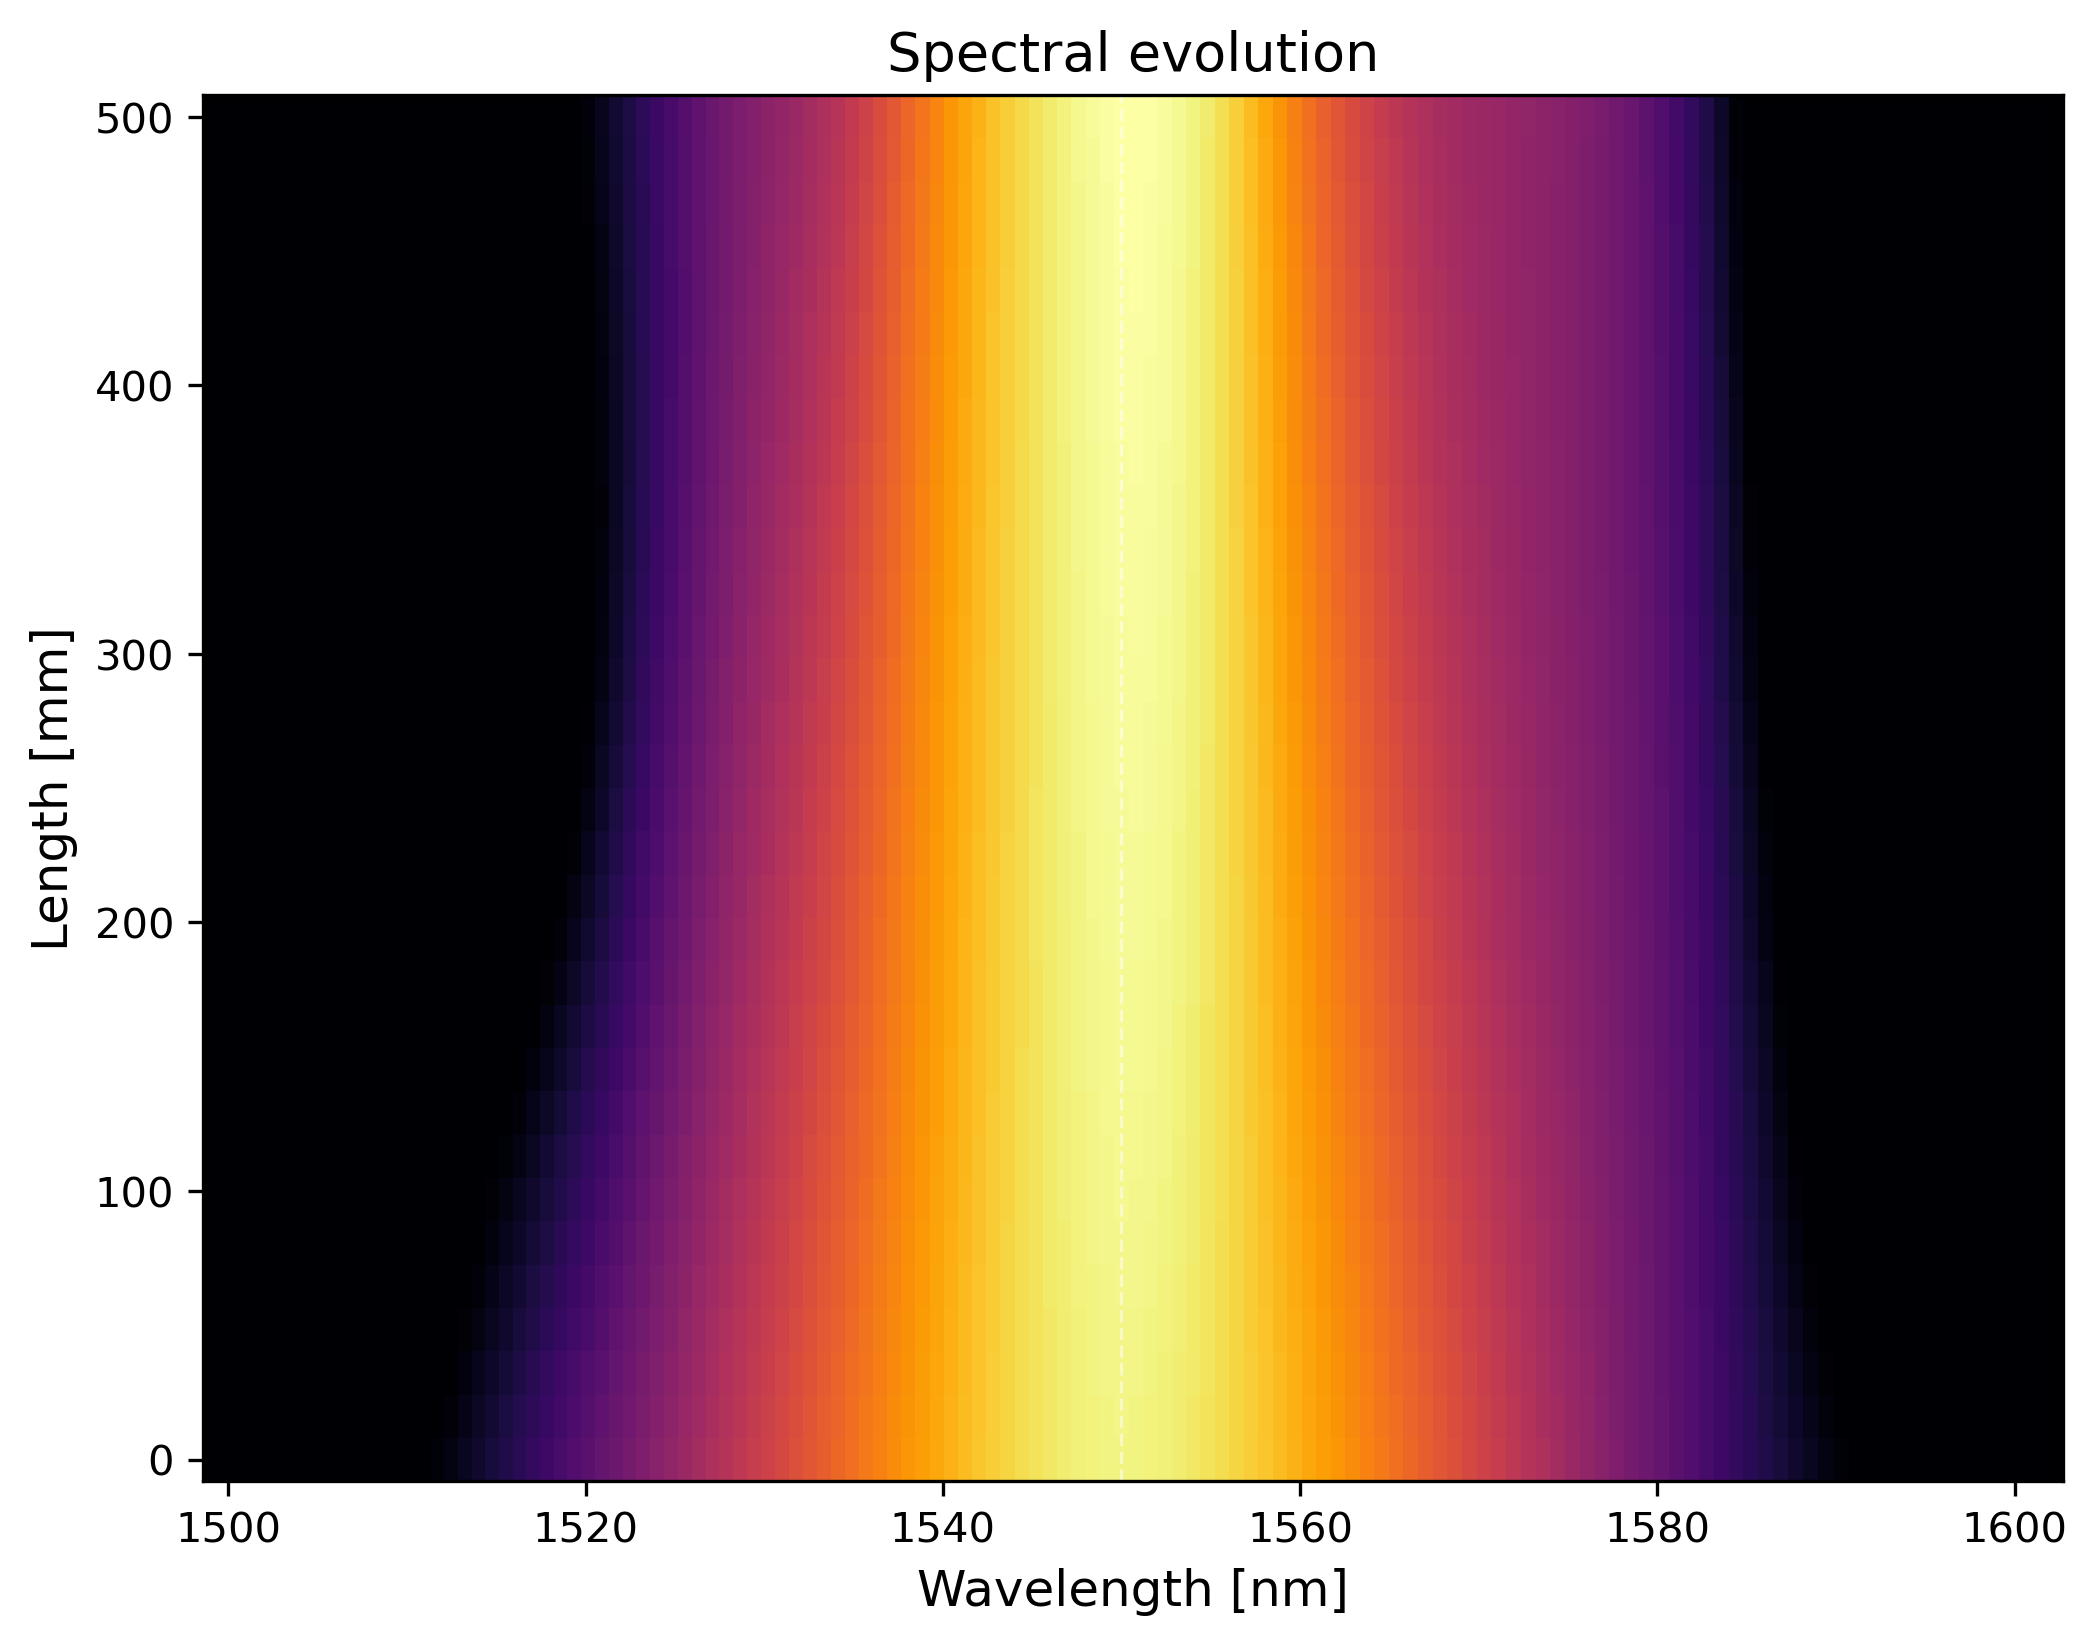
\includegraphics[height=0.31\textheight]{figures/deep_simple_profile_evolution.png}
\caption{Deep simple-looking mask. This is a striking native result, but the
stability tests show that its fixed-mask performance is fragile. It is better
treated as an initializer or basin clue than as a universal mask.}
\end{figure}

\begin{figure}[p]
\centering
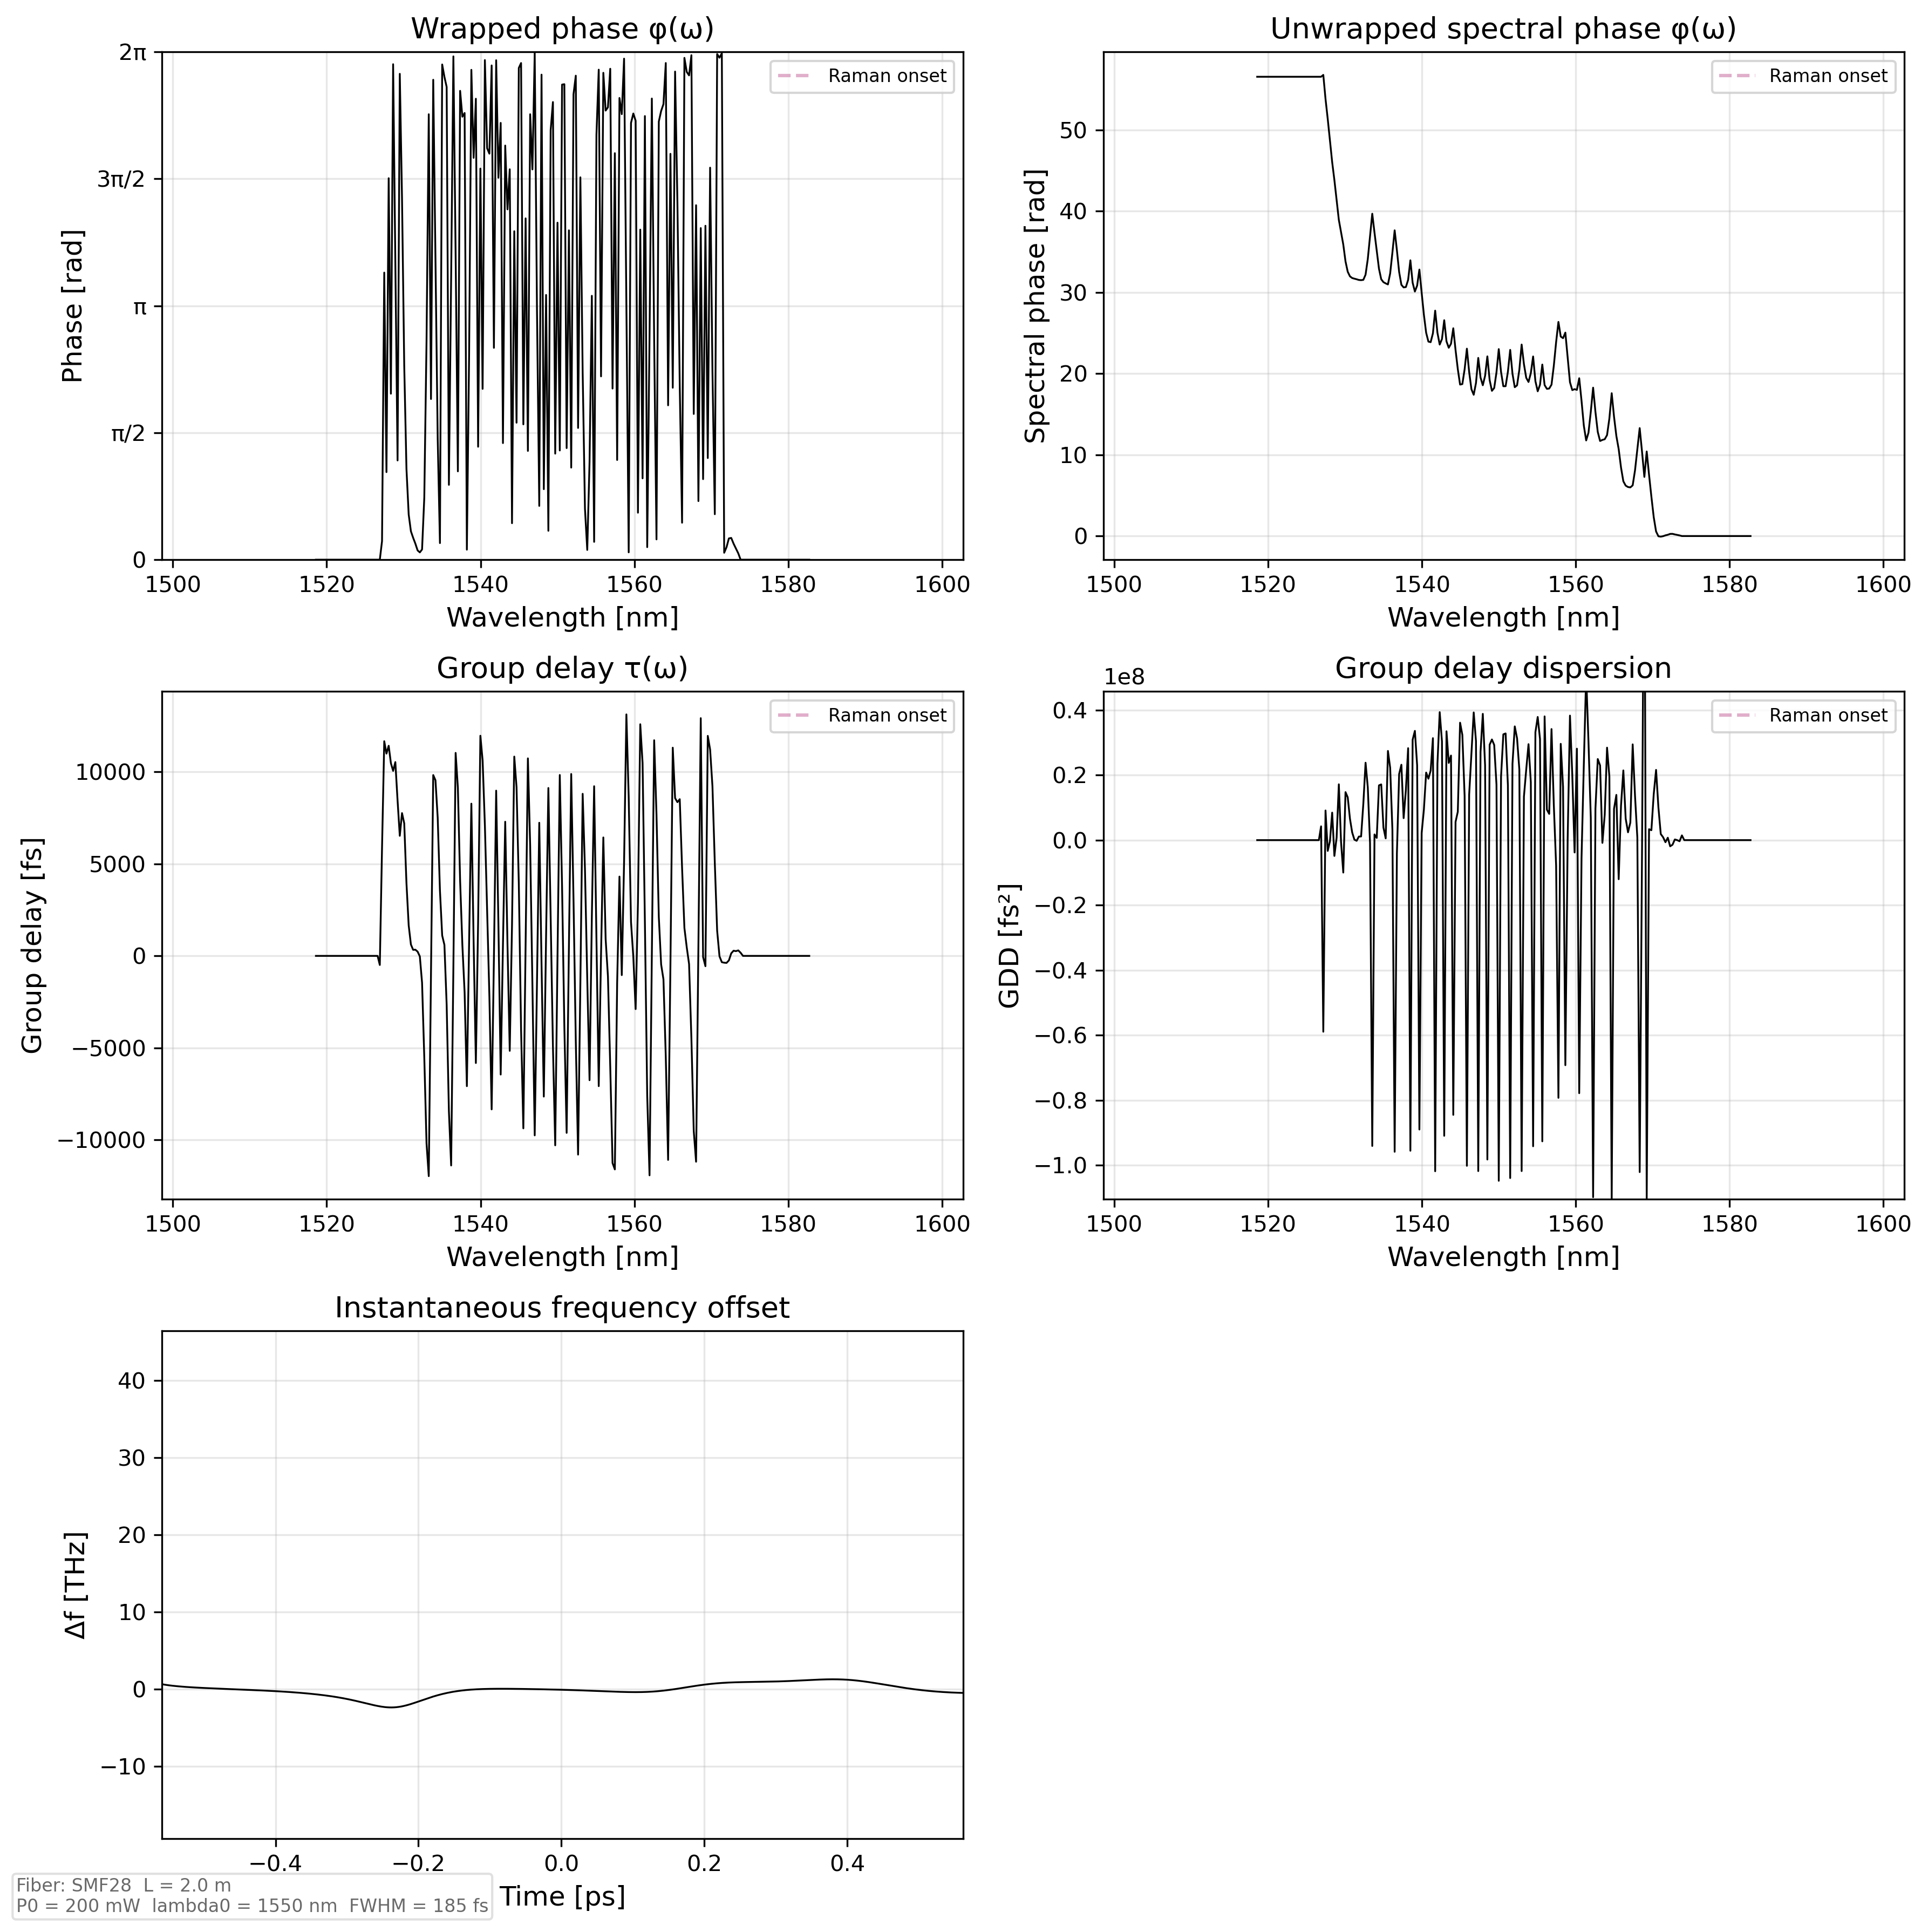
\includegraphics[height=0.47\textheight]{figures/deep_structured_profile_phase_diagnostic.png}
\par\vspace{0.5em}
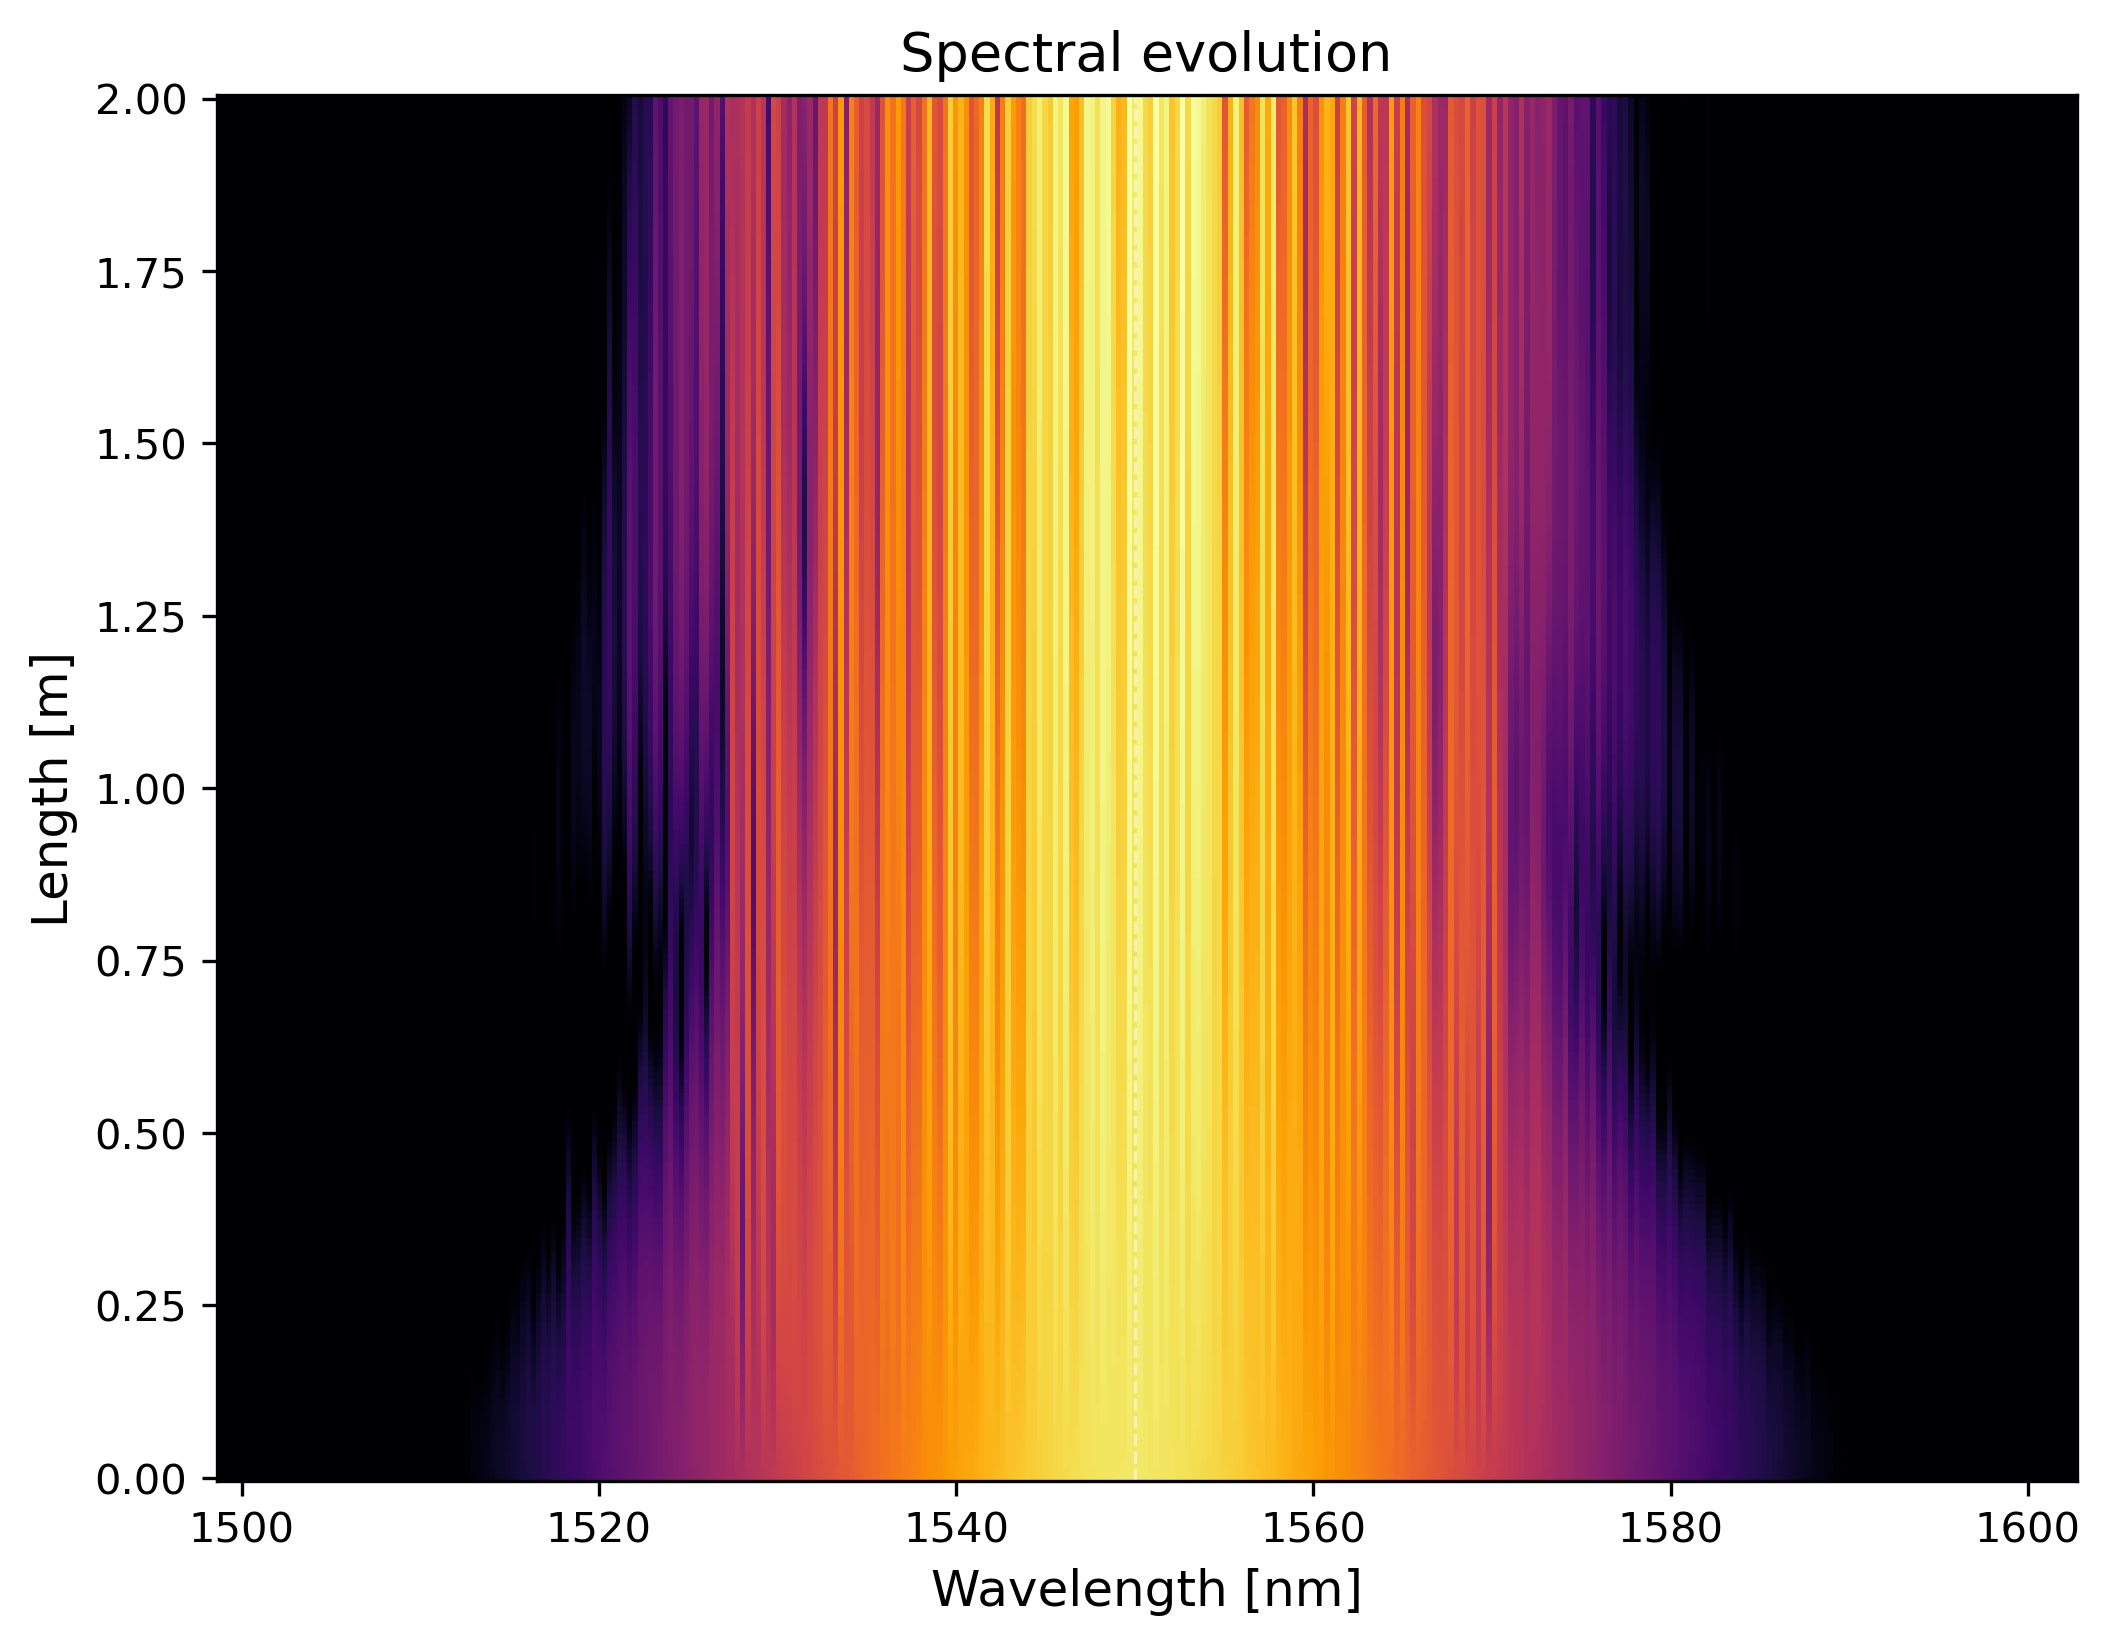
\includegraphics[height=0.31\textheight]{figures/deep_structured_profile_evolution.png}
\caption{Deep structured reduced-basis mask. This class reaches strong native
suppression, but its hardware-like perturbation losses are large.}
\end{figure}

\clearpage
\section{Interpretation}

The useful lesson is not that simple profiles always win. They do not. The
deepest native profiles are much deeper than the simple polynomial. The useful
lesson is that the simple profile is the cleanest baseline for a transferable
mechanism, while the deep profiles are evidence that much stronger local
suppression is possible.

That gives a better presentation structure:
\begin{itemize}
    \item \textbf{Mechanism story:} low-order chirp-like phase stretches and
    retimes the pulse, reducing Raman growth in a way that transfers.
    \item \textbf{Performance story:} richer phase structure can access much
    deeper suppression in the canonical setup.
    \item \textbf{Caution story:} the deepest masks are not automatically
    robust, transferable, or hardware-ready.
\end{itemize}

\subsection*{Intuition Check}

When presenting this, avoid saying ``the simple phase is the best.'' Say:
``The simple phase is the most explainable transferable baseline. The deep
profiles show what is possible locally. The open problem is to close the gap
between those two.''

\section{Presentation Capsule}

If this note becomes a transferability slide, the clean message is:
\begin{itemize}
    \item Simple, transferable, robust, and deepest are different design goals.
    \item The simple polynomial profile is useful because it is explainable and transfers well, not because it is the deepest native optimizer result.
    \item The deep structured masks show much stronger local suppression, but they are more fragile and less portable.
    \item The best presentation visual is the side-by-side tradeoff: simple transferable profile versus deep structured profile, each with its phase diagnostic and heat map.
\end{itemize}

\section{Limitations}

\textbf{One-trial robustness probes are screening tests.} Some forward probes
used one perturbation sample per setting. That is enough to flag major
fragility, but finalists need larger Monte Carlo checks.

\textbf{Hardware modeling is incomplete.} Pixelation, smoothing, wrapping, and
finite-bit masks are useful filters, but they are not a full pulse-shaper
calibration model.

\textbf{Transfer is not the same as warm-start success.} A mask can fail as a
fixed transfer but still be a strong initializer for reoptimization. Those
claims should be reported separately.

\textbf{Deep masks may still be physically meaningful.} Fragile does not mean
fake. It means the claim needs to be narrower unless robustness is improved.

\section{Reproduction Capsule}

The simple-profile and stability utilities are grouped into three small code
areas: simple-profile drivers, simple-candidate sweeps, and
stability/universality probes. The standard workflow is:
\begin{enumerate}
    \item produce or load candidate phase profiles;
    \item gauge-fix and compute simplicity metrics;
    \item evaluate fixed-mask transfer and perturbation probes;
    \item regenerate standard images for representative candidates;
    \item visually inspect the phase diagnostic and shaped/unshaped heat maps
    before using a candidate in a report.
\end{enumerate}

For any future finalist, the required evidence should include native
suppression, transfer matrix, noise curve, smoothing/pixelation survival,
wrapped-mask test, and a paired standard image page.

\section{Sources and References}

\begin{thebibliography}{9}
\bibitem{agrawal2019}
G. P. Agrawal. \textit{Nonlinear Fiber Optics}, 6th ed. Academic Press, 2019.
\url{https://www.sciencedirect.com/book/9780128170427/nonlinear-fiber-optics}

\bibitem{dudley2006}
J. M. Dudley, G. Genty, and S. Coen. ``Supercontinuum generation in photonic
crystal fiber.'' \textit{Reviews of Modern Physics}, 78, 1135--1184, 2006.
\url{https://doi.org/10.1103/RevModPhys.78.1135}

\bibitem{hult2007}
J. Hult. ``A fourth-order Runge-Kutta in the interaction picture method for
simulating supercontinuum generation in optical fibers.'' \textit{Journal of
Lightwave Technology}, 25(12), 3770--3775, 2007.
\url{https://doi.org/10.1109/JLT.2007.909373}

\bibitem{strickland1985}
D. Strickland and G. Mourou. ``Compression of amplified chirped optical
pulses.'' \textit{Optics Communications}, 56(3), 219--221, 1985.
\url{https://doi.org/10.1016/0030-4018(85)90120-8}

\bibitem{weiner2000}
A. M. Weiner. ``Femtosecond pulse shaping using spatial light modulators.''
\textit{Review of Scientific Instruments}, 71, 1929--1960, 2000.
\url{https://doi.org/10.1063/1.1150614}

\bibitem{gordon1986}
J. P. Gordon. ``Theory of the soliton self-frequency shift.'' \textit{Optics
Letters}, 11(10), 662--664, 1986. \url{https://doi.org/10.1364/OL.11.000662}

\bibitem{mitschke1986}
F. M. Mitschke and L. F. Mollenauer. ``Discovery of the soliton
self-frequency shift.'' \textit{Optics Letters}, 11(10), 659--661, 1986.
\url{https://doi.org/10.1364/OL.11.000659}
\end{thebibliography}

\end{document}
